% ---------------------------------------------------------------
% TEMPLATE TCC1 - SENAC SANTO AMARO
% ---------------------------------------------------------------
% Trabalho de Conclusão de Curso 1
% Elaborado para apresentação da proposta inicial do TCC
% Estrutura: 4 capítulos (Introdução, Revisão Bibliográfica,
%            Desenvolvimento, Referências Bibliográficas)
% ---------------------------------------------------------------

\documentclass[
    12pt,                % tamanho da fonte
    openright,           % capítulos começam em página ímpar
    oneside,             % para impressão em apenas um lado do papel
    a4paper,             % tamanho do papel
    english,             % idioma adicional
    brazil               % idioma principal
]{abntex2}

% ---------------------------------------------------------------
% PACOTES
% ---------------------------------------------------------------
\usepackage{lmodern}                % Fonte Latin Modern
\usepackage[T1]{fontenc}            % Seleção de códigos de fonte
\usepackage[utf8]{inputenc}         % Codificação do documento
\usepackage{lastpage}               % Usado pela Ficha catalográfica
\usepackage{indentfirst}            % Indenta o primeiro parágrafo
\usepackage{color}                  % Controle de cores
\usepackage{graphicx}               % Inclusão de gráficos
\usepackage{microtype}              % Melhorias de justificação
\usepackage{float}                  % Para posicionamento de figuras
\usepackage{tabularx}  
\usepackage{booktabs}               % Tabelas profissionais
\usepackage{multirow}               % Células mescladas em tabelas
\usepackage{longtable}              % Tabelas longas
\usepackage{amsmath,amssymb}        % Símbolos matemáticos
\usepackage{pgfgantt}               % Diagramas de Gantt
\usepackage[brazilian,hyperpageref]{backref}  % Páginas com citações
\usepackage[alf]{abntex2cite}       % Citações ABNT

% ---------------------------------------------------------------
% CONFIGURAÇÕES DO PDF
% ---------------------------------------------------------------
\makeatletter
\hypersetup{
    pdftitle={\@title},
    pdfauthor={\@author},
    pdfsubject={TCC1 - SENAC Santo Amaro},
    pdfcreator={LaTeX with abnTeX2},
    pdfkeywords={tcc}{senac}{santo amaro}{trabalho de conclusão},
    colorlinks=true,        % false: links em caixas; true: links coloridos
    linkcolor=blue,         % cor dos links internos
    citecolor=blue,         % cor dos links para bibliografia
    filecolor=magenta,      % cor dos links para arquivos
    urlcolor=blue,
    bookmarksdepth=4
}
\makeatother

% ---------------------------------------------------------------
% CONFIGURAÇÕES DE APARÊNCIA DO PDF FINAL
% ---------------------------------------------------------------
\definecolor{blue}{RGB}{41,5,195}

% ---------------------------------------------------------------
% INFORMAÇÕES DO DOCUMENTO
% ---------------------------------------------------------------
\titulo{Detecção de Intenção Implícita para Ativação de Assistentes de Voz em Ambientes Controlados}
\autor{Phelipe Pereira de Souza}
\local{São Paulo}
\data{2026}
\orientador{Prof. Thyago Conchado Quintas}
% \coorientador{Prof. Nome do Coorientador} % Descomente se houver coorientador

\instituicao{%
  SENAC -- Serviço Nacional de Aprendizagem Comercial
  \par
  Unidade Santo Amaro
  \par
  Bacharelado em Ciência da Computação
}

\tipotrabalho{Trabalho de Conclusão de Curso I}

\preambulo{Proposta de Trabalho de Conclusão de Curso apresentado ao SENAC Santo Amaro como requisito parcial para aprovação na disciplina de TCC1 do Bacharelado em Ciência da Computação.}

% ---------------------------------------------------------------
% COMPILA O ÍNDICE
% ---------------------------------------------------------------
\makeindex

% ---------------------------------------------------------------
% INÍCIO DO DOCUMENTO
% ---------------------------------------------------------------
\begin{document}

% Seleciona o idioma do documento
\selectlanguage{brazil}

% Retira espaço extra obsoleto entre as frases
\frenchspacing

% ---------------------------------------------------------------
% ELEMENTOS PRÉ-TEXTUAIS
% ---------------------------------------------------------------
\pretextual

% ---------------------------------------------------------------
% CAPA
% ---------------------------------------------------------------
\imprimircapa

% ---------------------------------------------------------------
% FOLHA DE ROSTO
% ---------------------------------------------------------------
\imprimirfolhaderosto

% ---------------------------------------------------------------
% RESUMO
% ---------------------------------------------------------------
% \begin{resumo}

    
% \vspace{\onelineskip}

% \noindent
% % \textbf{Palavras-chave}: palavra1. palavra2. palavra3. palavra4. palavra5.
% \end{resumo}

% ---------------------------------------------------------------
% LISTA DE ILUSTRAÇÕES
% ---------------------------------------------------------------
\pdfbookmark[0]{\listfigurename}{lof}
\listoffigures*
\cleardoublepage

% ---------------------------------------------------------------
% LISTA DE TABELAS
% ---------------------------------------------------------------
\pdfbookmark[0]{\listtablename}{lot}
\listoftables*
\cleardoublepage

% ---------------------------------------------------------------
% LISTA DE ABREVIATURAS E SIGLAS
% ---------------------------------------------------------------
\begin{siglas}
  \item[ASR] \textit{Automatic Speech Recognition} (Reconhecimento Automático de Fala)
  \item[DDSD] \textit{Device-Directed Speech Detection} (Detecção de Fala Direcionada ao Dispositivo)
  \item[EER] \textit{Equal Error Rate} (Taxa de Erro Igual)
  \item[HCI] \textit{Human-Computer Interaction} (Interação Humano-Computador)
  \item[HMM] \textit{Hidden Markov Model} (Modelo Oculto de Markov)
  \item[LLM] \textit{Large Language Model} (Modelo de Linguagem de Grande Porte)
  \item[LR] \textit{Logistic Regression} (Regressão Logística)
  \item[ML] \textit{Machine Learning} (Aprendizado de Máquina)
  \item[NLP] \textit{Natural Language Processing} (Processamento de Linguagem Natural)
  \item[NLU] \textit{Natural Language Understanding} (Compreensão de Linguagem Natural)
  \item[SVM] \textit{Support Vector Machines} (Máquinas de Vetores de Suporte)
  \item[TF-IDF] \textit{Term Frequency-Inverse Document Frequency} (Frequência do Termo - Inverso da Frequência nos Documentos)
  \item[TTS] \textit{Text-to-Speech} (Síntese de Fala)
  \item[VAD] \textit{Voice Activity Detection} (Detecção de Atividade de Voz)
  \item[WER] \textit{Word Error Rate} (Taxa de Erro de Palavras)
\end{siglas}
\cleardoublepage

% ---------------------------------------------------------------
% SUMÁRIO
% ---------------------------------------------------------------
\pdfbookmark[0]{\contentsname}{toc}
\tableofcontents*
\cleardoublepage

% ---------------------------------------------------------------
% ELEMENTOS TEXTUAIS
% ---------------------------------------------------------------
\textual

% ===============================================================
% CAPÍTULO 1 - INTRODUÇÃO
% ===============================================================
\chapter{Introdução}
\label{cap:introducao}

Nas últimas décadas, os assistentes de voz tornaram-se componentes cada vez mais presentes no cotidiano, incorporados a \textit{smartphones}, alto-falantes inteligentes, \textit{wearables} e sistemas de automação residencial~\cite{Jurafsky2024}. Esses sistemas permitem que usuários interajam com dispositivos computacionais por meio de comandos de voz, facilitando a execução de tarefas como busca de informações, controle de dispositivos domésticos e gerenciamento de atividades. O mercado global de assistentes de voz foi avaliado em US\$ 7,35 bilhões em 2024 e projeta-se que alcance US\$ 33,74 bilhões até 2030, com taxa de crescimento anual composta de 26,5\%, o que evidencia a escala e a relevância dessa tecnologia, conforme ilustrado no gráfico de projeção da Figura~\ref{fig:market}~\cite{NMSC2025}.

\begin{figure}[htb]       
    \centering           
    \caption{Projeção de crescimento do mercado global de assistentes virtuais de voz (2024--2030).}
    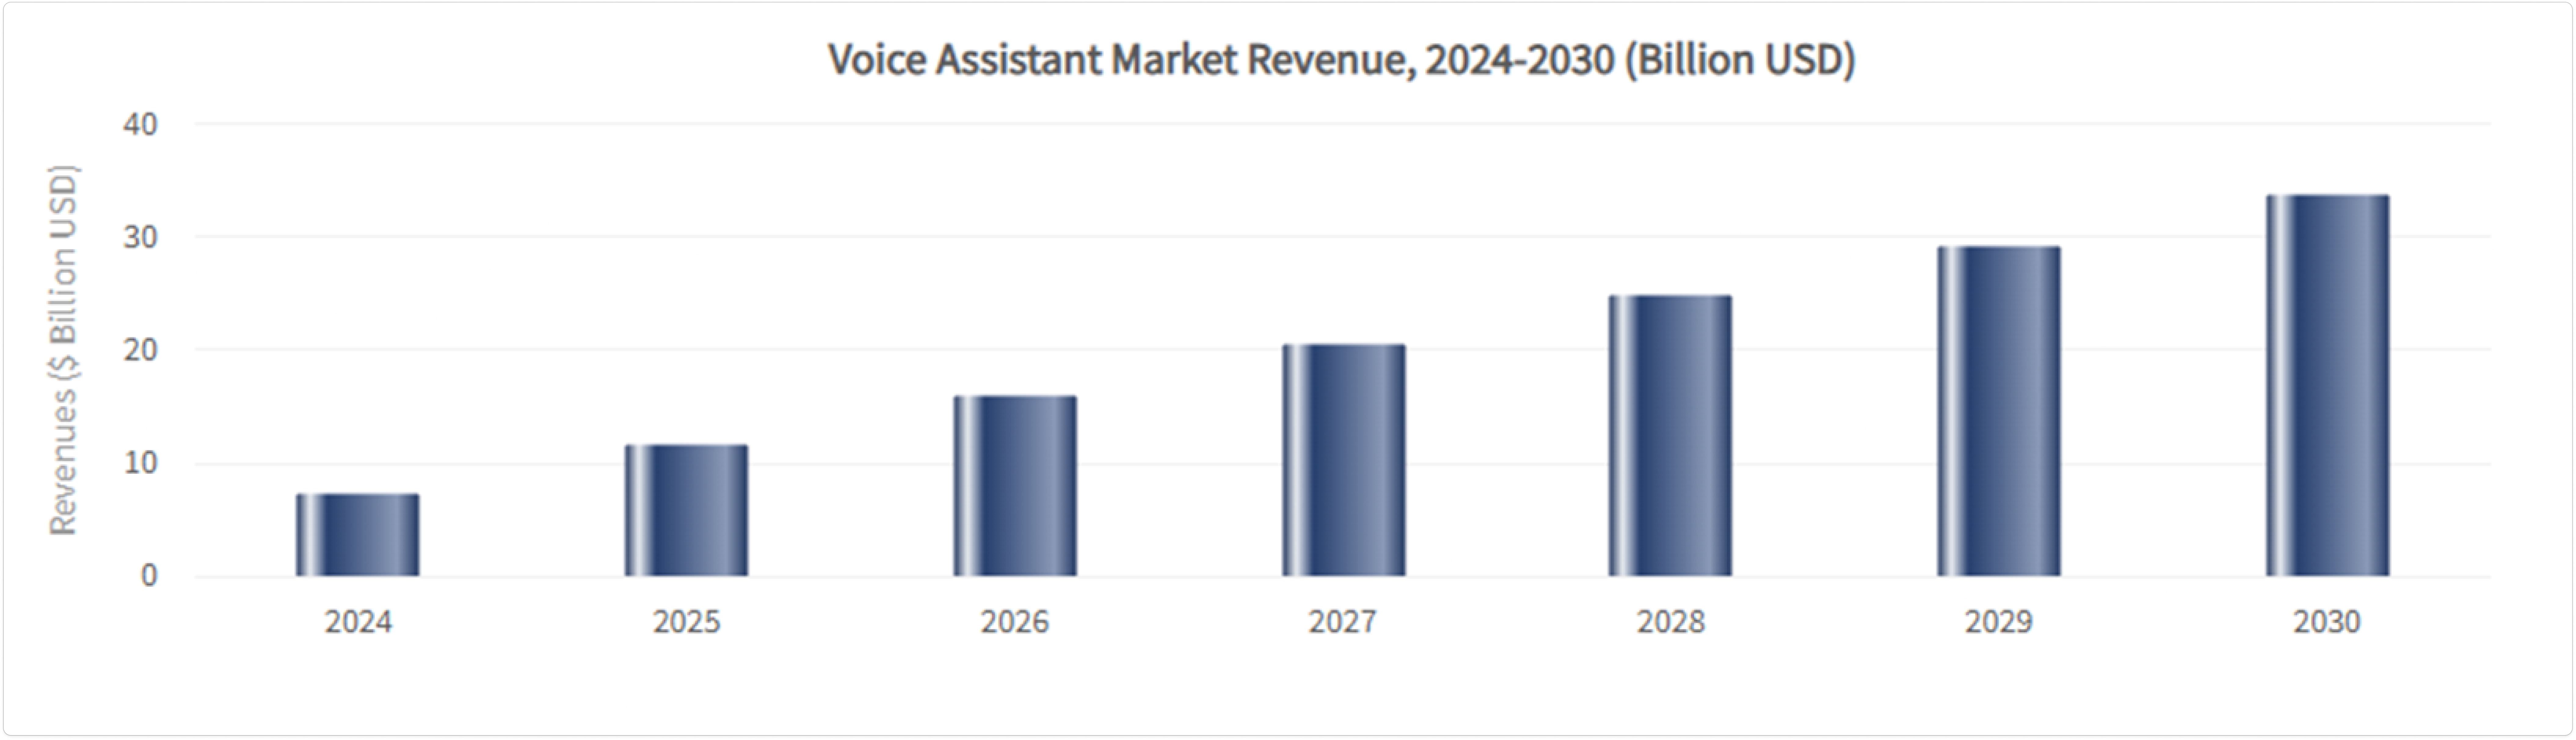
\includegraphics[width=1.0\textwidth]{market.png} 
    \fonte{Next Move Strategy Consulting (2025).}
    \label{fig:market}
\end{figure}

Na maioria dos sistemas atuais, a interação com assistentes de voz é iniciada por meio de palavras de ativação explícitas, conhecidas como \textit{wake-words} ou \textit{hotwords}, tais como ``Hey Siri'', ``Alexa'' ou ``Ok Google''. Essas expressões atuam como um mecanismo de gatilho que sinaliza ao sistema o desejo do usuário de iniciar uma interação. Do ponto de vista técnico, essa abordagem é eficaz, pois permite reduzir o processamento contínuo de áudio e minimizar ativações indevidas \cite{Garg2021}. No entanto, a dependência de \textit{wake-words} impõe limitações significativas à naturalidade da comunicação humano-computador, tornando a interação menos fluida e intuitiva quando comparada ao diálogo humano \cite{Nie2021}.

Em interações humanas cotidianas, comandos e solicitações são frequentemente expressos de forma implícita, inseridos naturalmente no fluxo da conversação, sem a necessidade de uma palavra específica para iniciar a comunicação \cite{Weld2022}. Em contraste, os sistemas baseados em \textit{wake-words} são vulneráveis ao fenômeno de ativações falsas por palavras foneticamente semelhantes, conhecido como \textit{FakeWake} \cite{Chen2021}. Esse problema compromete a qualidade da experiência do usuário, evidenciando as limitações da abordagem atual para a viabilização de uma interação verdadeiramente natural e intuitiva.

Nesse cenário, surge a área de pesquisa denominada \textit{Device-Directed Speech Detection} (traduzido como Detecção de Fala Direcionada ao Dispositivo, referenciado pela sigla DDSD), que visa determinar automaticamente se uma fala é direcionada a um assistente virtual, mesmo na ausência de uma palavra de ativação explícita, ou se faz parte de uma conversa entre humanos \cite{Mallidi2018, Wagner2024}. Essa abordagem possibilita interações mais naturais e fluidas, reduzindo a necessidade de gatilhos verbais explícitos (\textit{wake-words}) e representando um avanço significativo rumo a uma comunicação humano-computador mais intuitiva e semelhante ao diálogo cotidiano.

Este trabalho investiga a viabilidade da DDSD em português brasileiro por meio de uma abordagem baseada exclusivamente no nível textual. O sistema proposto opera com transcrições de fala obtidas via Reconhecimento Automático de Fala (do inglês \textit{Automatic Speech Recognition}, referido pela sigla ASR), e aplica técnicas de Processamento de Linguagem Natural (do inglês \textit{Natural Language Processing}, referido pela sigla NLP) e Aprendizado de Máquina (do inglês \textit{Machine Learning}, referido pela sigla ML) para classificar automaticamente se uma fala é direcionada ao dispositivo ou faz parte de uma conversa incidental entre humanos. O foco deste trabalho reside na etapa de classificação de intenção, tratando o ASR como um módulo de pré-processamento encarregado de gerar as transcrições textuais que servirão de entrada para o classificador.

% ---------------------------------------------------------------

\section{Cenário motivador}
\label{sec:cenario}

\begin{figure}[htb]       
    \centering           
    \caption{Cenário ilustrativo de Detecção de Fala Direcionada ao Dispositivo (DDSD).}
    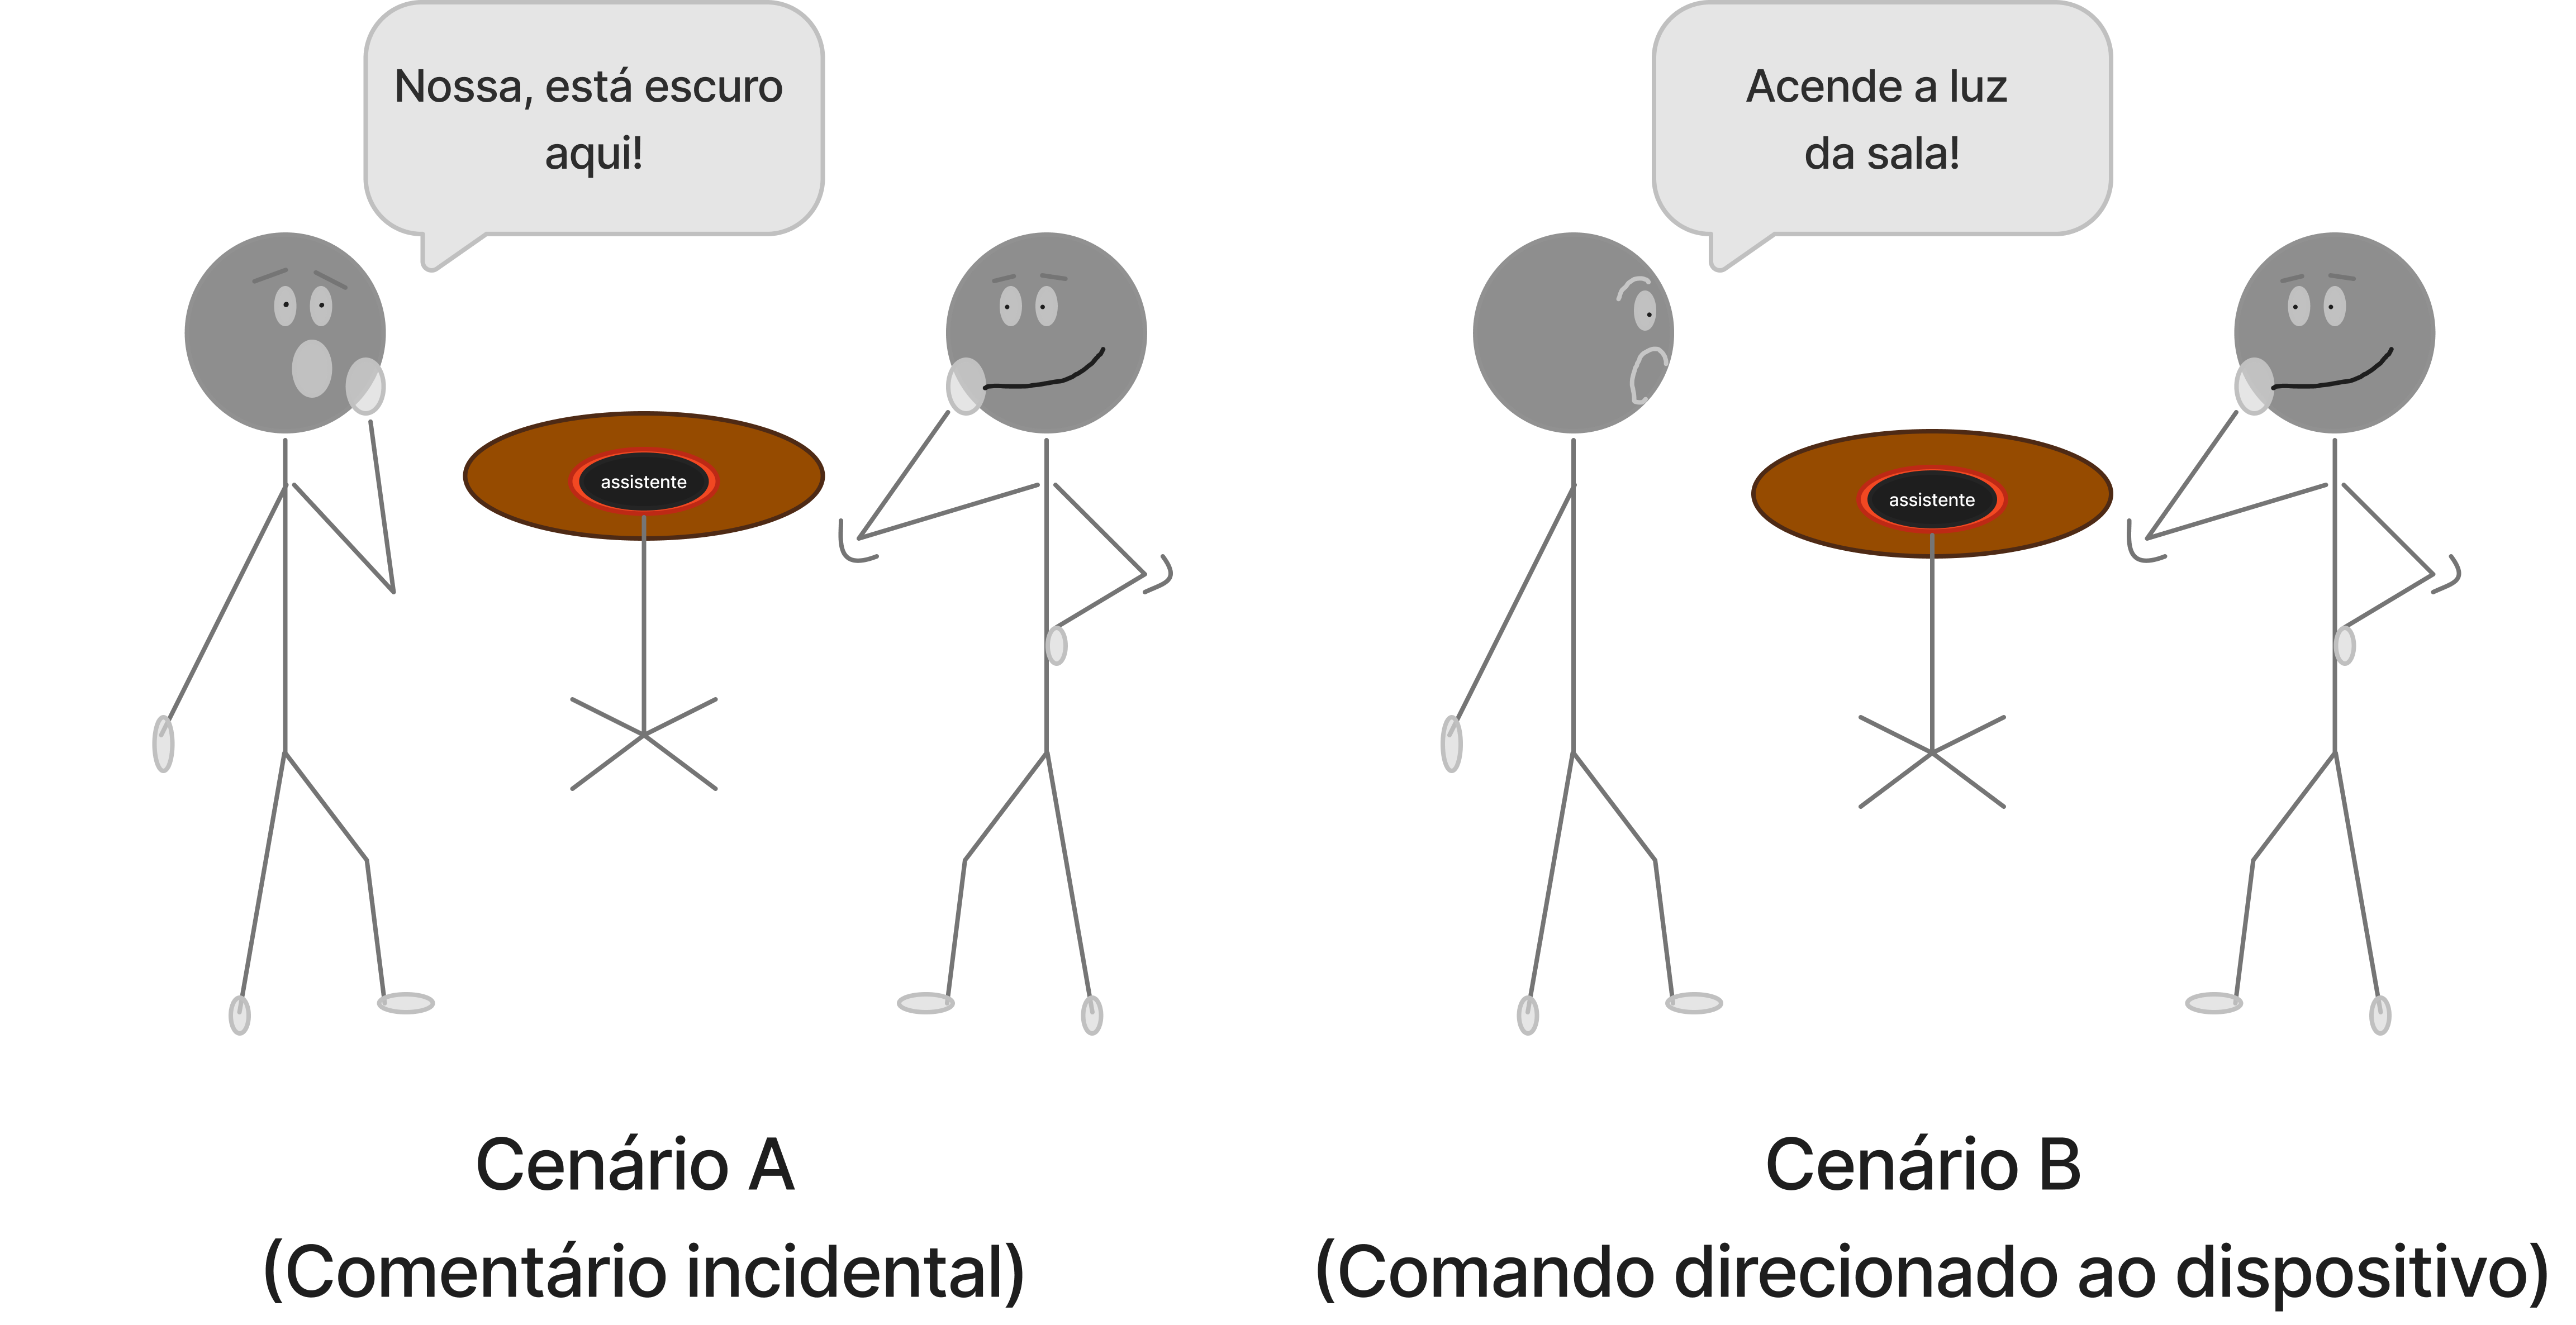
\includegraphics[width=0.75\textwidth]{cenario.png} 
    \fonte{Elaborado pelo autor (2026).}
    \label{fig:cenario}
\end{figure}

Para ilustrar a complexidade e a relevância do problema, considere o cenário prático apresentado na Figura~\ref{fig:cenario}: em uma sala de estar, duas pessoas conversam informalmente na presença de um assistente de voz ativo. Uma delas comenta, em tom casual: ``nossa, está escuro aqui''. O sistema não deve acionar a iluminação, visto que o enunciado constitui apenas um comentário incidental e não uma instrução direcionada. Momentos depois, a mesma pessoa olha para o dispositivo e diz: ``acende a luz da sala''. Nesse cenário, mesmo na ausência de uma \textit{wake-word}, o assistente deve ser capaz de reconhecer a fala como claramente direcionada a ele.

Esse cenário ilustra as três classes de enunciados que o sistema precisa distinguir: (i) comandos implícitos direcionados ao dispositivo (DD, do inglês \textit{Device-Directed}), como ``acende a luz''; (ii) comentários incidentais e conversas paralelas, classificados como não direcionados ao dispositivo (NDD, do inglês \textit{Non-Device-Directed}), como ``nossa, está escuro aqui''; e (iii) enunciados ambíguos (AMB), cujo direcionamento depende estritamente do contexto extraverbal, como ``apaga a luz, por favor'', que pode ser direcionado tanto a um interlocutor humano quanto ao assistente. O problema de DDSD consiste precisamente em classificar automaticamente esses enunciados em tempo real, sem depender de \textit{wake-words} explícitas \cite{Mallidi2018, Wagner2024}.

% ---------------------------------------------------------------
\section{Contexto}
\label{sec:contexto}

O desenvolvimento de assistentes de voz tem sido impulsionado por avanços significativos nas áreas de ASR e NLP. Modelos de última geração, como o Whisper \cite{Radford2023}, representam marcos importantes ao viabilizar a transcrição de áudio com elevada precisão e robustez em múltiplos idiomas. Em 2024, a OpenAI disponibilizou o Whisper Large V3 Turbo, uma versão otimizada que reduz o número de camadas do decodificador de 32 para 4, mantendo desempenho próximo ao modelo completo com ganho de velocidade de aproximadamente 6 vezes \cite{Jeffries2024, Bevilacqua2024}. Essa versão é adotada neste trabalho como módulo principal de ASR, por oferecer o melhor equilíbrio entre precisão e eficiência para o português brasileiro. Na literatura, outras alternativas relevantes incluem o Whispy \cite{Bevilacqua2024}, que adapta o Whisper para cenários de fluxo contínuo (\textit{streaming}), e modelos compactos como o Moonshine \cite{Jeffries2024}, voltados para execução em dispositivos embarcados.

Especificamente para o português brasileiro, modelos baseados na arquitetura Wav2Vec 2.0 \cite{Grosman2021}, ajustados com dados nacionais, também têm demonstrado resultados relevantes na literatura, representando alternativas para lidar com as variações fonéticas e prosódicas do idioma.

Simultaneamente, os desenvolvimentos em NLP foram revolucionados pela arquitetura Transformer \cite{Vaswani2017}, que serve de base para os modernos LLMs (Modelos de Linguagem de Grande Porte, do inglês \textit{Large Language Models}). No âmbito nacional, o BERTimbau \cite{Souza2020} consolidou o uso de Transformers especializados em português brasileiro para tarefas de compreensão textual, sendo adotado neste trabalho como classificador principal de intenção. Mais recentemente, modelos como Albertina \cite{Rodrigues2023} e DeBERTinha \cite{Abonizio2023} introduziram abordagens altamente eficientes em termos de parâmetros e representação semântica, sendo considerados como alternativas a serem exploradas caso o cronograma permita. Ademais, LLMs generativos como o Sabiá \cite{Pires2023} ampliaram as competências de geração textual para o idioma, sendo empregado neste trabalho para a geração sintética de enunciados direcionados ao dispositivo na construção do corpus de experimentos.

Torna-se necessário delimitar o papel específico de cada família de modelos no escopo deste projeto: o Whisper Large V3 Turbo atua como módulo principal de ASR para a conversão de fala em texto, enquanto Moonshine e Wav2Vec 2.0 são mencionados como referências da literatura. Os modelos de linguagem pré-treinados, com destaque para o BERTimbau como classificador principal e DeBERTinha e Albertina como alternativas, constituem o núcleo da decisão de DDSD textual. Por fim, o Sabiá é empregado como ferramenta de geração sintética de dados para a construção do corpus. A Tabela~\ref{tab:tecnologias} sintetiza essa distribuição de responsabilidades.

\begin{table}[H]
\caption{Mapeamento de tecnologias e seus papéis no trabalho}
\label{tab:tecnologias}
\begin{tabular}{lll}
\toprule
\textbf{Tecnologia} & \textbf{Papel no trabalho} & \textbf{Será implementada?} \\
\midrule
Whisper Large V3 Turbo & ASR - geração de transcrição     & Sim (principal) \\
Moonshine              & ASR - referência bibliográfica   & Não \\
Wav2Vec 2.0 PT-BR      & ASR - referência bibliográfica   & Não \\
BERTimbau              & Classificador textual (principal) & Sim \\
DeBERTinha             & Classificador textual (alternativo) & Opcional \\
Albertina              & Classificador textual (alternativo) & Opcional \\
TF-IDF + SVM/LR        & Baseline clássico                & Sim \\
Sabiá                  & Geração sintética de dados DD    & Sim \\
\bottomrule
\end{tabular}
\fonte{Elaborado pelo autor (2026).}
\end{table}

Pesquisas recentes em DDSD têm investigado abordagens focadas no nível do texto para mitigar as limitações de sistemas puramente acústicos. Trabalhos recentes \cite{Wagner2024, Dighe2024} demonstraram que aplicar classificadores baseados em Transformers sobre as hipóteses de transcrição geradas por sistemas de ASR configura-se como uma estratégia robusta para inferir o direcionamento do enunciado. Expandindo essa premissa, \citeonline{Rudovic2024} evidenciaram como a semântica textual permite decodificar intenções implícitas em fluxos de diálogo contínuo, corroborando a viabilidade técnica da modelagem puramente linguística do sinal de áudio transcrito.

% ---------------------------------------------------------------
\section{Justificativa}
\label{sec:justificativa}

A crescente presença de assistentes de voz em diferentes dispositivos computacionais evidencia a relevância de pesquisas voltadas à melhoria da Interação Humano-Computador (conhecida por HCI, do inglês \textit{Human-Computer Interaction}). Apesar dos avanços significativos em ASR e NLP, a maioria dos sistemas atuais ainda depende de palavras de ativação explícitas, que podem comprometer a naturalidade e a fluidez da comunicação \cite{Mallidi2018}. Em ambientes com interações dinâmicas e frequentes, a necessidade de invocar repetidamente o dispositivo pode gerar fadiga no usuário e prejudicar a experiência de uso \cite{Nie2021}. Diante disso, o desenvolvimento de sistemas de DDSD apresenta-se como uma abordagem relevante para reduzir a dependência de palavras de ativação explícitas e promover interações mais fluidas e intuitivas \cite{Wagner2024}.

Sob a perspectiva acadêmica, o estudo de métodos alternativos de ativação baseados em intenção implícita situa-se na convergência do processamento de áudio, NLP e HCI. Embora a literatura aponte que a fusão multimodal (acústica e textual) resulte em menores taxas de erro de ativação \cite{Wagner2024}, a implementação de sistemas multimodais demanda alto poder computacional, processos complexos de sincronização temporal de sinais e grandes volumes de dados rotulados em ambas as modalidades, o que impõe barreiras severas para a implantação em dispositivos de borda ou com recursos computacionais restritos \cite{Xu2024}.

Adicionalmente, identifica-se uma lacuna geográfica e linguística na literatura: os principais estudos sobre DDSD concentram-se quase exclusivamente no idioma inglês, com forte dependência de características acústicas e prosódicas nativas daquela língua \cite{Norouzian2019, Krishna2023}. O português brasileiro, apesar de ser um dos idiomas mais falados do mundo, apresenta-se sub-representado nesse campo de pesquisa, carecendo de estudos focados na decodificação de padrões de direcionamento de fala adaptados à sua realidade gramatical e cultural.

Embora o ecossistema nacional tenha presenciado o surgimento de recursos linguísticos robustos, como o BERTimbau \cite{Souza2020} e corpora públicos de fala (ex.: CORAA ASR \cite{CORAA2023}, NURC-SP \cite{NURCSP2025}, TAGARELA \cite{Tagarela2026}), tais bases destinam-se prioritariamente a tarefas de transcrição fonética e reconhecimento acústico tradicional. Verifica-se, portanto, uma escassez de corpora especificamente anotados com fins de detecção de direcionamento de voz (DD vs NDD) em português brasileiro, constituindo um gargalo para a pesquisa científica e o desenvolvimento de soluções práticas para DDSD nesse idioma.

Nesse cenário, este trabalho busca contribuir para o preenchimento dessa lacuna ao investigar a viabilidade técnica de uma abordagem de DDSD puramente textual, alimentada por hipóteses de transcrição geradas por sistemas de ASR e operacionalizada por meio de modelos baseados em Transformer pré-treinados para o português brasileiro. A escolha exclusiva pela modalidade textual fundamenta-se em três pilares metodológicos: (i) a superioridade dos modelos baseados em atenção para capturar nuances semânticas e intenções implícitas em tarefas de classificação de enunciados curtos \cite{Weld2022}; (ii) as evidências empíricas de que o sinal linguístico presente em transcrições automáticas carrega alto poder discriminativo para diferenciar comandos de conversações casuais \cite{Wagner2024, Dighe2024}. e (iii)  o ganho de modularidade e isolamento arquitetural, o que facilita a comparação rigorosa com baselines lineares e viabiliza a mensuração precisa do impacto de ruídos e erros de transcrição de áudio \cite{Dighe2024}.

% ---------------------------------------------------------------

\section{Hipótese de pesquisa}
\label{sec:hipotese}

A hipótese central deste trabalho é a seguinte: 

\textit{Sob condições de ambiente controlado, modelos de linguagem pré-treinados para o português brasileiro, aplicados sobre transcrições geradas por sistemas de ASR, alcançam desempenho estatisticamente superior a baselines lineares tradicionais, constituídos pela representação TF-IDF combinada com SVM ou LR, avaliados sobre o mesmo corpus sob as métricas de F1-score, acurácia e EER, comprovando a viabilidade técnica da abordagem puramente textual para a tarefa de DDSD em português brasileiro.}

Essa conjectura encontra sustentação nos fundamentos apresentados na Seção~\ref{sec:fundamentos}: a viabilidade da classificação puramente textual sobre hipóteses de ASR \cite{Wagner2024}, a superioridade de arquiteturas Transformer em tarefas de classificação de intenção \cite{Weld2022} e o desempenho comprovado de modelos especializados no português brasileiro, como o BERTimbau \cite{Souza2020} e o DeBERTinha \cite{Abonizio2023}. 

A validação dessa hipótese será realizada por meio de experimentos controlados no TCC2, utilizando um corpus anotado especificamente para a tarefa de DDSD em português brasileiro, com protocolo de validação cruzada e comparação rigorosa entre o modelo baseado em Transformer e os \textit{baselines} lineares definidos nos Objetivos Específicos.

% ---------------------------------------------------------------
\section{Objetivos}
\label{sec:objetivos}

\subsection{Objetivo principal}

O objetivo principal desta pesquisa consiste em avaliar a viabilidade técnica e o desempenho de modelos de linguagem pré-treinados para o português brasileiro aplicados à DDSD, operando sob transcrições puramente textuais geradas por sistemas de ASR, de modo a verificar se essa abordagem supera estatisticamente os \textit{baselines} lineares compostos por TF-IDF associado a SVM ou LR, nas métricas de F1-score, acurácia e EER.

\subsection{Objetivos específicos}

Para que o objetivo principal seja alcançado, foram definidos os seguintes objetivos específicos:

\begin{enumerate}
    \item Construir e validar um corpus balanceado de sentenças em português brasileiro, anotadas com base no direcionamento de fala (DD e NDD) sob critérios explícitos de anotação e rigorosos de exclusão, a partir de adaptações de corpora públicos (CORAA ASR \cite{CORAA2023}, NURC-SP \cite{NURCSP2025} e TAGARELA \cite{Tagarela2026}) e enunciados sintetizados controlados gerados por LLMs.

    \item Implementar, ajustar (fine-tuning) e avaliar o modelo BERTimbau \cite{Souza2020} na tarefa de classificação binária de DDSD, confrontando empiricamente seus resultados com um \textit{baseline} composto pela representação vetorial TF-IDF aliada a SVM ou LR, utilizando hipóteses de transcrição geradas por ASR (1-best e/ou n-best).

    \item Analisar o impacto gerado por erros e ruídos de transcrição automática no classificador semântico de intenções, mapeando o desempenho comparativo entre transcrições manuais e automáticas e estabelecendo a correlação estatística entre a \textit{Word Error Rate} (traduzida como Taxa de Erro de Palavras, referenciada pela sigla WER) das saídas do ASR e o decaimento de desempenho do classificador textual \cite{Dighe2024}.
\end{enumerate}

% ---------------------------------------------------------------

\section{Limitações do trabalho}
\label{sec:limitacoes}

Esta proposta apresenta restrições de escopo e limitações do desenho experimental adotado, explicitadas a seguir para contextualizar os resultados.

A primeira limitação refere-se à exclusividade da modalidade de entrada. O modelo proposto analisa estritamente informações do domínio textual das transcrições, omitindo características prosódicas, acústicas ou paralinguísticas (entonação, velocidade e pausas) comprovadamente relevantes para a DDSD \cite{Norouzian2019, Krishna2023}. Embora seja uma escolha deliberada para estabelecer uma base textual robusta antes do desenvolvimento multimodal, assume-se o risco de o sistema apresentar menor sensibilidade em cenários com ruídos acústicos acentuados ou variações expressivas de tom.

A segunda limitação reside no impacto dos erros de transcrição gerados pelo ASR. Como a entrada do classificador depende diretamente da transcrição gerada pelo Whisper, erros fonéticos ou omissões podem corromper as estruturas gramaticais e semânticas analisadas pelo Transformer, especialmente em falas com sotaque, ruído de fundo ou vocabulário incomum \cite{Bevilacqua2024}. O impacto desses erros será analisado como parte dos experimentos, mas representa uma fonte de variabilidade não completamente controlável. A comparação entre transcrições manuais e automáticas, prevista no terceiro objetivo específico, buscará quantificar essa degradação.

A terceira limitação está associada à construção, representatividade e escala do corpus experimental. Diante da ausência de bases especificamente anotadas para DDSD em português brasileiro, torna-se necessária a construção de um corpus próprio em ambiente controlado, combinando dados reais fragmentados e geração sintética assistida por LLMs. Tal estratégia implica restrições em termos de escala, espontaneidade conversacional, diversidade sociolinguística regional e variabilidade dialetal. Consequentemente, o corpus resultante não contemplará toda a complexidade e variabilidade da fala espontânea em contextos reais \cite{CORAA2023}, o que pode limitar a capacidade de generalização dos resultados.

Por fim, esta pesquisa não contempla aspectos relacionados à infraestrutura de implantação em ambientes produtivos, como latência de ponta a ponta, processamento contínuo em fluxo no dispositivo (\textit{on-device streaming}), armazenamento de sinais de áudio, segurança de dados e privacidade. O foco repousa exclusivamente na análise experimental e estatística da viabilidade da classificação textual em ambiente laboratorial controlado, delegando a estudos futuros os desafios regulatórios e arquiteturais de privacidade, processamento local e mecanismos de consentimento do usuário \cite{Chen2021}.

% ===============================================================
% CAPÍTULO 2 - REVISÃO BIBLIOGRÁFICA
% ===============================================================
\chapter{Revisão Bibliográfica}
\label{cap:revisao}

Este capítulo estabelece o embasamento teórico e tecnológico da pesquisa proposta. Inicialmente, descreve-se a metodologia de seleção dos trabalhos consultados. O referencial teórico, na sequência, percorre os paradigmas de interação por voz, desde os mecanismos tradicionais de ativação baseados em \textit{wake-words} até as abordagens emergentes de Detecção de Fala Direcionada ao Dispositivo (do inglês \textit{Device-Directed Speech Detection}, referida pela sigla DDSD). Os fundamentos técnicos são então aprofundados, com ênfase na arquitetura Transformer, nos modelos de linguagem pré-treinados para o português brasileiro e nas métricas de avaliação. Por fim, analisam-se os trabalhos mais diretamente relacionados ao tema, identificando lacunas que esta pesquisa busca preencher.

\section{Metodologia da pesquisa bibliográfica}
\label{sec:metodologia_pesquisa}

\begin{figure}[htb]       
    \centering           
    \caption{Fluxo de seleção de estudos para a revisão bibliográfica.}
    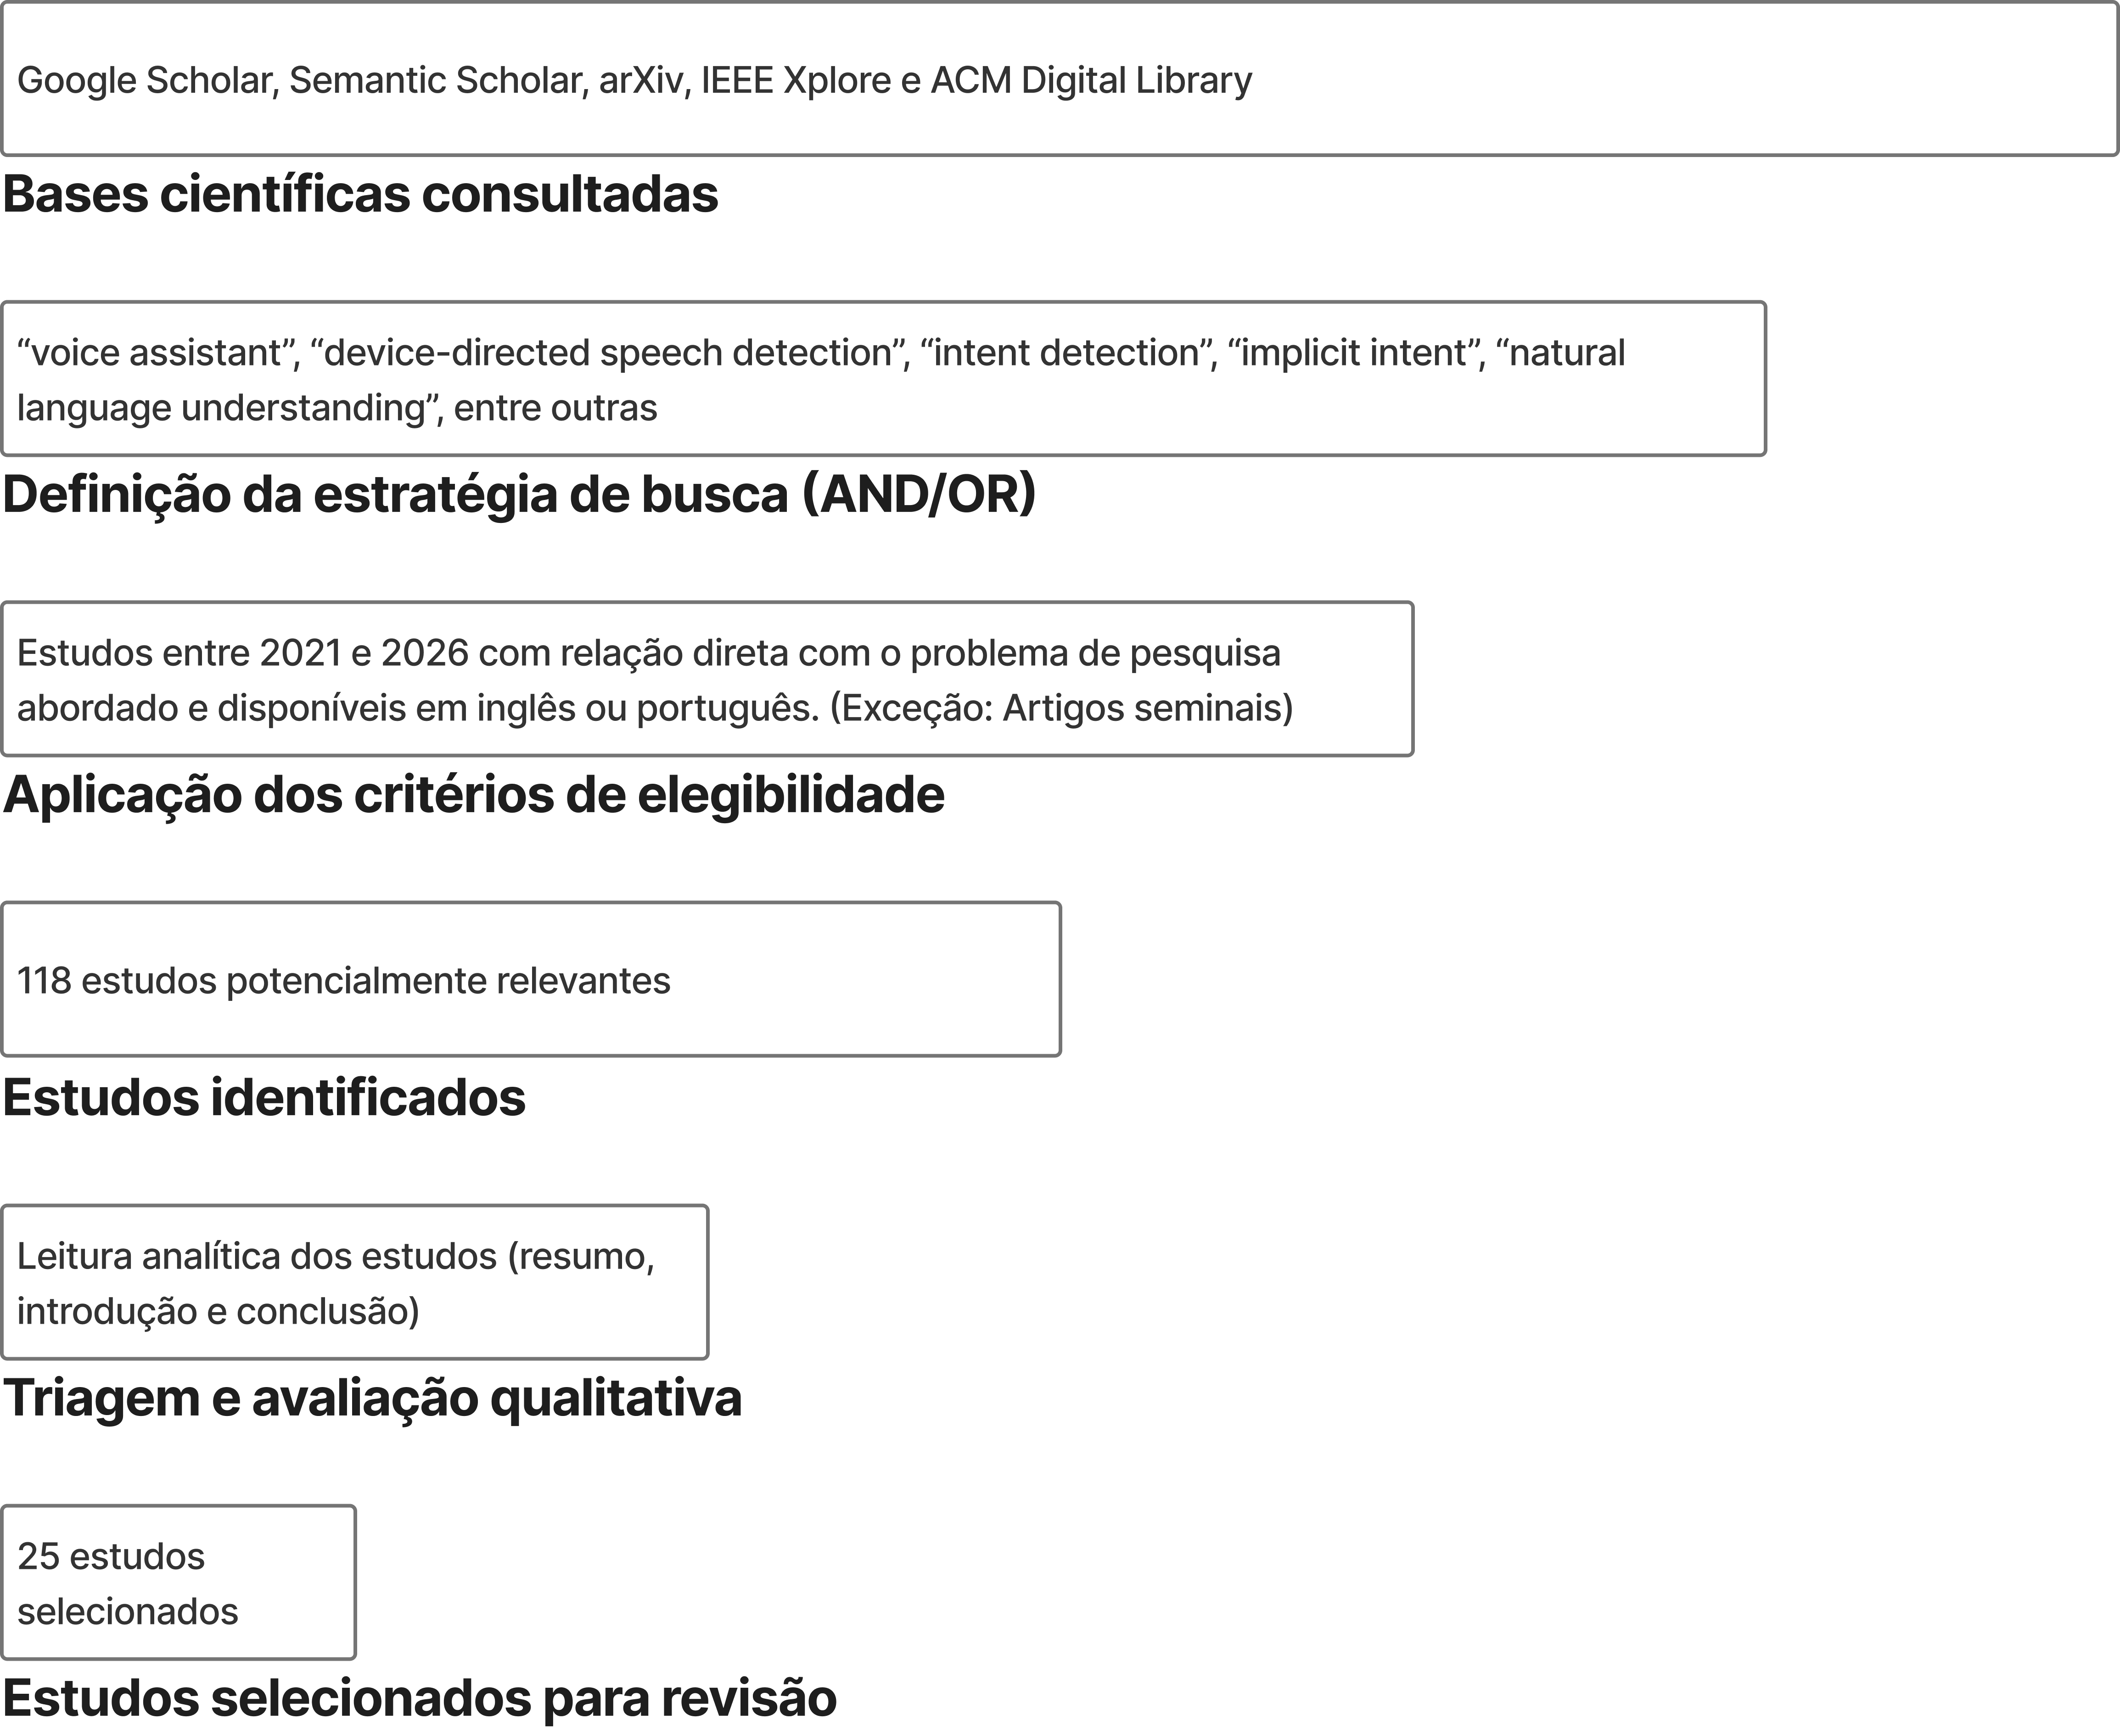
\includegraphics[width=0.85\textwidth]{funil.png} 
    \fonte{Elaborado pelo autor (2026).}
    \label{fig:funil}
\end{figure}

A pesquisa bibliográfica foi conduzida de forma estruturada com o objetivo de identificar trabalhos científicos relevantes sobre detecção de intenção em linguagem natural, assistentes virtuais baseados em voz, DDSD e técnicas de aprendizado de máquina aplicadas ao reconhecimento e classificação de comandos de voz.

Foram consultadas bases de dados acadêmicas amplamente utilizadas na área de Computação, incluindo Google Scholar, Semantic Scholar, arXiv, IEEE Xplore e ACM Digital Library. Essas plataformas foram selecionadas por concentrarem artigos científicos, pré-publicações e trabalhos revisados por pares com abrangência nas áreas de processamento de fala, linguagem natural e aprendizado de máquina.

As buscas utilizaram combinações de palavras-chave em inglês, tais como: \textit{``voice assistant''}, \textit{``device-directed speech detection''}, \textit{``intent detection''}, \textit{``keyword spotting''}, \textit{``implicit intent''}, \textit{``wake-word''}, \textit{``false trigger mitigation''}, \textit{``natural language understanding''} e \textit{``voice command classification''}. Essas expressões foram combinadas por meio de operadores booleanos (AND, OR) para ampliar ou restringir os resultados conforme necessário.

Como critérios de inclusão, foram considerados: (a) trabalhos publicados entre 2021 e 2026; (b) disponibilidade nos idiomas inglês ou português; (c) relação direta com o problema de pesquisa, priorizando-se artigos que apresentassem experimentos, métodos de classificação ou avaliações de sistemas de interação por voz. Como exceção, foram incluídos artigos seminais anteriores ao período definido, por representarem contribuições fundamentais para a área, como os trabalhos sobre a arquitetura Transformer \cite{Vaswani2017} e o BERT \cite{Devlin2019}.

Como critérios de exclusão, foram desconsiderados: (a) trabalhos publicados antes de 2021, exceto os seminais; (b) artigos sem relação direta com detecção de intenção, DDSD ou classificação de comandos de voz; (c) trabalhos duplicados entre as bases consultadas.

O processo de seleção ocorreu em duas etapas, conforme ilustrado na Figura~\ref{fig:funil}. Na triagem inicial, foram identificados 118 artigos potencialmente relevantes com base na leitura de título e resumo. Na etapa de afunilamento, a análise em maior profundidade resultou na seleção de 27 trabalhos para compor a fundamentação teórica, os trabalhos relacionados e as referências deste estudo. Adicionalmente, foram incluídos 7 artigos seminais anteriores a 2021, entre os quais se destacam os trabalhos sobre a arquitetura Transformer \cite{Vaswani2017}, o BERT \cite{Devlin2019}, o BERTimbau \cite{Souza2020} e os primeiros estudos de DDSD \cite{Mallidi2018, Norouzian2019}. Dessa forma, o conjunto final de referências selecionadas para este trabalho foi composto por 34 artigos.

% ---------------------------------------------------------------
\section{Referencial teórico}
\label{sec:referencial}

O referencial teórico apresenta os conceitos que sustentam este trabalho, estabelecendo um contraponto entre o modelo predominante de interação com assistentes virtuais baseado em comandos explícitos (\textit{wake-words}) e a busca por interações mais naturais por meio da DDSD. A organização dos tópicos segue o fluxo típico de processamento de um assistente virtual baseado em voz, desde a captura e identificação da fala destinada ao sistema, passando pela transcrição do áudio, até a compreensão semântica da intenção do usuário.

% ---------------------------------------------------------------

\subsection{Assistentes virtuais e interação por voz}

A evolução da Interação Humano-Computador (conhecida por HCI, do inglês \textit{Human-Computer Interaction}) tem avançado das interfaces puramente gráficas e táteis em direção a interfaces conversacionais e ubíquas. Nesse contexto, os assistentes virtuais baseados em voz consolidaram-se como agentes computacionais capazes de interpretar linguagem natural, processar requisições e executar tarefas automatizadas, mediando a relação entre o usuário e ecossistemas de serviços digitais.

De acordo com \citeonline{Jurafsky2024}, assistentes virtuais são sistemas que integram tecnologias de ASR (Reconhecimento Automático de Fala, do inglês \textit{Automatic Speech Recognition}), Compreensão de Linguagem Natural (NLU, do inglês \textit{Natural Language Understanding}) e Síntese de Fala (TTS, do inglês \textit{Text-to-Speech}) para viabilizar interações fluidas entre humanos e dispositivos. O funcionamento típico segue um \textit{pipeline} sequencial: (i)~captura do sinal de áudio; (ii)~Detecção de Atividade de Voz (VAD, do inglês \textit{Voice Activity Detection}); (iii)~ASR; (iv)~NLU; e (v)~geração da resposta ou execução da ação solicitada.

Na maioria dos sistemas comerciais, essas etapas são precedidas por um módulo de detecção de \textit{wake-word}, que atua como gatilho para iniciar o processamento mais custoso \cite{Garg2021}. Essa arquitetura permite que o assistente permaneça em modo de baixo consumo até ser explicitamente invocado. A relevância dessas tecnologias é corroborada pelo crescimento acelerado do mercado global de assistentes de voz, conforme apresentado no Capítulo~\ref{cap:introducao} \cite{NMSC2025}.

A eficácia da interação, no entanto, depende da capacidade do sistema de identificar quando sua intervenção é solicitada. Em ambientes cotidianos, onde a fala humana é simultaneamente direcionada a outras pessoas e a dispositivos, surge o desafio de distinguir intenções implícitas, tema central deste trabalho.

% ---------------------------------------------------------------

\subsection{Detecção de Atividade de Voz (VAD)}

A Detecção de Atividade de Voz (VAD) é a primeira etapa de processamento após a captura do áudio, sendo responsável por identificar os segmentos do sinal que contêm fala humana e separá-los de trechos de silêncio, ruído de fundo e sons não verbais \cite{Li2021}. Ao descartar trechos sem fala, o VAD reduz o volume de dados processado pelos módulos subsequentes (ASR e NLU), diminuindo o consumo computacional e a latência, aspectos críticos em dispositivos embarcados e de borda.

Em ambientes controlados, a tarefa é relativamente simples, baseada em limiares de energia ou características acústicas tradicionais. Em cenários reais, a robustez torna-se um desafio, e modelos baseados em aprendizado profundo têm alcançado resultados superiores \cite{Li2021}. A qualidade da detecção impacta diretamente as etapas posteriores do \textit{pipeline}. Um VAD muito permissivo gera ativações desnecessárias, enquanto um VAD restritivo demais pode descartar falas relevantes. Dessa forma, o equilíbrio entre sensibilidade e especificidade constitui um aspecto importante para o desempenho de assistentes de voz. Embora o VAD esteja fora do escopo de implementação deste trabalho, seu papel como pré-requisito funcional do \textit{pipeline} justifica sua menção no referencial.

% ---------------------------------------------------------------

\subsection{Reconhecimento Automático de Fala (ASR)}

O Reconhecimento Automático de Fala (ASR) consiste na conversão de um sinal de áudio contendo fala humana em texto legível por máquina \cite{Jurafsky2024}. No contexto de assistentes virtuais, o ASR atua como ponte entre o processamento do sinal acústico e os módulos de compreensão semântica.

Historicamente, os sistemas de ASR baseavam-se em abordagens híbridas que combinavam Modelos de Markov Ocultos (HMM, do inglês \textit{Hidden Markov Models}) com modelos de linguagem estatísticos \cite{Jurafsky2024}. Essas abordagens dominaram a área por décadas, mas apresentavam limitações na modelagem de dependências temporais longas e no aproveitamento de grandes volumes de dados. A partir da década de 2010, o aprendizado profundo trouxe avanços significativos, inicialmente com redes recorrentes (RNN, LSTM) e convolucionais, e posteriormente com a arquitetura Transformer \cite{Vaswani2017}, que permitiu saltos expressivos de desempenho. Modelos contemporâneos, como o Whisper \cite{Radford2023}, atingiram robustez elevada em múltiplos idiomas ao serem treinados com supervisão fraca em corpora massivos. Os detalhes técnicos do Whisper e de outros modelos de ASR empregados neste trabalho são apresentados na Seção~\ref{sec:fundamentos}.

A qualidade dos sistemas de ASR é comumente mensurada pela métrica \textit{Word Error Rate} (traduzida como Taxa de Erro de Palavras, referenciada pela sigla WER), que calcula a proporção de palavras erradas, substituídas, deletadas ou inseridas em relação a uma transcrição de referência. Em aplicações de assistentes virtuais, erros de transcrição propagam-se diretamente para as etapas de classificação de intenção, o que torna o WER um indicador relevante para o desempenho final do sistema.

% ---------------------------------------------------------------

\subsection{Wake-words: mecanismo, vantagens e limitações}

As \textit{wake-words} (também denominadas \textit{hotwords} ou palavras de ativação) constituem o mecanismo predominante de ativação em assistentes virtuais comerciais. Trata-se de expressões pré-definidas, tais como ``Hey Siri'', ``Alexa'', ``Ok Google'' e ``Hey Bixby'', que funcionam como gatilho para despertar o sistema do estado de espera e iniciar o processamento da solicitação do usuário \cite{Garg2021}.

Do ponto de vista técnico, a detecção de \textit{wake-words} é realizada por um módulo de \textit{keyword spotting} que opera continuamente no dispositivo com consumo energético reduzido. Esse módulo permanece ativo mesmo quando os componentes mais custosos do \textit{pipeline} (ASR e NLU) estão inativos, ativando-os somente após a detecção positiva da palavra de ativação \cite{Garg2021, Kundu2023}.

Essa abordagem oferece vantagens relevantes. Do ponto de vista energético, é eficiente e adequada para dispositivos alimentados por bateria \cite{Shin2023}. Contribui também para a preservação da privacidade, uma vez que o processamento em nuvem só é iniciado após a ativação explícita \cite{Nie2021}. Além disso, minimiza o processamento desnecessário de áudio ambiente.

No entanto, o mecanismo de \textit{wake-words} apresenta limitações. Do ponto de vista da HCI, impõe um padrão rígido e artificial de comunicação que contrasta com a naturalidade do diálogo humano \cite{Nie2021}. Uma vulnerabilidade técnica relevante é o fenômeno \textit{FakeWake}, em que expressões foneticamente semelhantes à \textit{wake-word} ativam inadvertidamente o sistema. \citeonline{Chen2021} desenvolveram um gerador automático de \textit{fuzzy words} capaz de produzir 965 expressões que acionavam indevidamente oito dos principais assistentes do mercado, comprometendo usabilidade e privacidade. 

Para mitigar os falsos gatilhos, foram propostas técnicas de mitigação de falsos acionamentos (FTM, do inglês \textit{False Trigger Mitigation}). \citeonline{Garg2021} apresentaram uma arquitetura baseada em Transformer com processamento em fluxo contínuo, capaz de suprimir até 95\% dos falsos positivos utilizando apenas um segundo de áudio contextual após a ativação. Apesar dos avanços, essas soluções adicionam complexidade ao sistema e não eliminam a necessidade de uma ativação explícita inicial, motivando o desenvolvimento de alternativas como a DDSD.

% ---------------------------------------------------------------

\subsection{Detecção de Fala Direcionada ao Dispositivo (DDSD)}

A Detecção de Fala Direcionada ao Dispositivo (DDSD) é definida como a tarefa de classificação binária que visa determinar automaticamente se um enunciado é intencionalmente direcionado a um assistente virtual ou se faz parte de uma conversa incidental entre humanos \cite{Mallidi2018, Wagner2024}.

Diferentemente do mecanismo de \textit{wake-words}, a DDSD busca permitir interações mais naturais, aproximando a comunicação humano-computador do padrão conversacional humano e superando as limitações de rigidez e fricção cognitiva discutidas na subseção anterior \cite{Nie2021}.

As pesquisas na área têm evoluído em duas frentes: abordagens multimodais e abordagens unimodais (baseadas em áudio ou texto). As soluções multimodais combinam informações acústicas, textuais, prosódicas e, em alguns casos, visuais. \citeonline{Wagner2024} demonstraram que a fusão de características acústicas, hipóteses do decodificador ASR e representações textuais processadas por LLMs (Modelos de Linguagem de Grande Porte, do inglês \textit{Large Language Models}) pode reduzir a taxa de erro em até 61\% frente a modelos unimodais. \citeonline{Krishna2023} exploraram a combinação de características verbais com informações prosódicas não verbais (entonação, ritmo e pausas), obtendo melhorias na taxa de falsa aceitação. Em outra vertente, \citeonline{Nie2021} propuseram um sistema multimodal integrando informações visuais (detecção facial e rastreamento labial) com características acústicas. Do ponto de vista exclusivamente acústico, \citeonline{Norouzian2019} investigaram o uso de mecanismos de atenção para classificar enunciados como dirigidos ou não ao sistema, evidenciando o potencial de \textit{features} espectrais combinadas com redes neurais de atenção.

Embora as abordagens multimodais obtenham melhor desempenho em cenários complexos, demandam maior poder computacional, sincronização precisa entre modalidades e grandes volumes de dados anotados multimodalmente, o que limita sua viabilidade em dispositivos com recursos restritos \cite{Wagner2024}. 

Nesse contexto, abordagens baseadas exclusivamente em texto, que utilizam transcrições geradas por ASR como entrada, têm sido exploradas como alternativa viável na literatura recente, embora permaneçam menos estudadas do que as soluções acústicas e multimodais. Essas soluções oferecem maior simplicidade arquitetural, modularidade e interpretabilidade, especialmente em idiomas com poucos recursos anotados, como o português brasileiro. Estudos recentes demonstram que as representações textuais extraídas de hipóteses ASR contêm sinal discriminativo relevante para a detecção de intenção implícita \cite{Dighe2024, Wagner2024}.

% ---------------------------------------------------------------

\subsection{Processamento de Linguagem Natural e classificação de intenção}

O Processamento de Linguagem Natural (do inglês \textit{Natural Language Processing}, referido pela sigla NLP) compreende o conjunto de técnicas computacionais destinadas à análise, compreensão e geração de linguagem humana em formato textual \cite{Jurafsky2024}. No contexto de assistentes virtuais, a subárea de Compreensão de Linguagem Natural (NLU) é responsável por extrair o significado semântico e a intenção do usuário a partir das transcrições geradas pelo ASR \cite{Weld2022}.

Dado um enunciado do usuário, o objetivo é identificar a intenção subjacente, ou seja, qual ação o sistema deve realizar \cite{Weld2022}. Essa tarefa é frequentemente combinada com o preenchimento de \textit{slots} (\textit{slot filling}), responsável por extrair os parâmetros necessários para a execução da ação (ex.: ``Defina um alarme para as 8 horas'' $\rightarrow$ intenção: ``criar alarme''; slot: horário = ``8 horas'').

Historicamente, os sistemas de classificação de intenção baseavam-se em regras manuais e padrões lexicais. Métodos estatísticos, como Máquinas de Vetores de Suporte (SVM), tornaram-se predominantes na sequência \cite{Manning2008}. Foi, contudo, a partir da introdução da arquitetura Transformer \cite{Vaswani2017} e, especialmente, do modelo BERT \cite{Devlin2019} que a área experimentou avanço expressivo. Em levantamento abrangente, \citeonline{Weld2022} concluem que modelos pré-treinados baseados em Transformers superam consistentemente abordagens anteriores em tarefas de detecção de intenção, tanto em precisão quanto em generalização.

A principal vantagem dos modelos pré-treinados reside na capacidade de realizar \textit{fine-tuning} com quantidades relativamente pequenas de dados rotulados \cite{Devlin2019}, característica particularmente atrativa para idiomas com poucos recursos linguísticos. A classificação de intenção constitui o núcleo da abordagem textual proposta para a DDSD, a partir das transcrições geradas pelo ASR, o sistema busca identificar se o enunciado carrega uma intenção direcionada ao dispositivo, mesmo na ausência de \textit{wake-words} explícitas.

\subsection{Modelos baseados em Transformers}

A arquitetura Transformer, proposta por \citeonline{Vaswani2017}, representou um dos principais marcos do NLP ao substituir recorrência e convoluções pelo mecanismo de \textit{atenção multi-cabeça} como principal componente para modelar dependências em sequências textuais. A partir dessa arquitetura, \citeonline{Devlin2019} propuseram o BERT (\textit{Bidirectional Encoder Representations from Transformers}), que introduziu o pré-treinamento bidirecional profundo e demonstrou ganhos expressivos em diversas tarefas de compreensão textual. O detalhamento técnico dessas arquiteturas, incluindo as formulações matemáticas do mecanismo de atenção e o processo de \textit{fine-tuning}, é apresentado na Seção~\ref{sec:fundamentos}.

No contexto do português brasileiro, \citeonline{Souza2020} desenvolveram o BERTimbau, versão do BERT pré-treinada especificamente para o idioma, com resultados superiores aos modelos multilíngues em tarefas como classificação textual e reconhecimento de entidades. Modelos mais recentes, como a DeBERTinha \cite{Abonizio2023} e a Albertina \cite{Rodrigues2023}, introduziram variantes com diferentes compromissos entre eficiência computacional e desempenho. Esses modelos são detalhados na Seção~\ref{sec:fundamentos} e constituem as opções de classificadores investigadas neste trabalho.

% ---------------------------------------------------------------
\section{Fundamentos}
\label{sec:fundamentos}

Esta seção detalha as tecnologias, algoritmos e metodologias específicas que serão empregadas no desenvolvimento da solução proposta. Diferentemente do referencial teórico, que contextualiza os conceitos gerais da área, os fundamentos aprofundam os aspectos técnicos diretamente utilizados na implementação.

% ---------------------------------------------------------------

\subsection{Arquitetura Transformer}

A arquitetura Transformer, introduzida por \citeonline{Vaswani2017}, eliminou a dependência de recorrência e convoluções, substituindo-as pelo mecanismo de atenção como principal componente para modelagem de sequências. Diferentemente das RNNs (Redes Neurais Recorrentes, do inglês \textit{Recurrent Neural Networks}), que processam sequências de forma sequencial, o Transformer processa todos os elementos da entrada simultaneamente, permitindo alto grau de paralelização. Embora variantes como LSTM (Memória de Longo e Curto Prazo, do inglês \textit{Long Short-Term Memory}) e GRU (Unidade Recorrente com Portão, do inglês \textit{Gated Recurrent Unit}) atenuem parcialmente o problema de dissipação de gradientes das RNNs tradicionais, essas arquiteturas ainda enfrentam limitações em dependências muito longas, que o Transformer supera por construção \cite{Vaswani2017}.

O componente central é o mecanismo de \textit{Self-Attention}. Para cada token da sequência, o modelo calcula três vetores: \textit{Query} (Q), \textit{Key} (K) e \textit{Value} (V). A atenção é obtida por:

\[
\text{Attention}(Q, K, V) = \text{softmax}\left(\frac{QK^T}{\sqrt{d_k}}\right)V
\]

onde \(d_k\) é a dimensão dos vetores de chave. Essa operação permite que cada token pondere a importância de todos os demais tokens da sequência. O fator de escala \(\sqrt{d_k}\) estabiliza os gradientes durante o treinamento.

Para aumentar a capacidade representacional, \citeonline{Vaswani2017} propuseram o \textit{Multi-Head Attention}, que executa o mecanismo de atenção em paralelo \(h\) vezes (tipicamente 8 ou 16 cabeças), cada uma com projeções lineares independentes de Q, K e V. As saídas são concatenadas e projetadas linearmente, permitindo que o modelo capture diferentes tipos de relações semânticas e sintáticas em uma mesma camada.

Como o Transformer não possui recorrência, é necessário injetar informação posicional por meio do \textit{Positional Encoding}. Os autores utilizaram funções seno e cosseno de diferentes frequências:

\[
PE_{(pos,2i)} = \sin\left(\frac{pos}{10000^{2i/d_{model}}}\right), \quad PE_{(pos,2i+1)} = \cos\left(\frac{pos}{10000^{2i/d_{model}}}\right)
\]

Esses valores são somados aos \textit{embeddings} dos tokens de entrada, fornecendo informação explícita sobre a ordem dos elementos.

A arquitetura completa é composta por blocos de \textit{Encoder} e \textit{Decoder}. Cada bloco do Encoder contém uma camada de Multi-Head Self-Attention seguida de uma rede \textit{feed-forward} posicionada (duas camadas lineares com ativação ReLU). O Decoder possui uma camada adicional de \textit{Cross-Attention} que recebe as saídas do Encoder. Conexões residuais e normalização de camada (\textit{layer normalization}) são aplicadas em torno de cada subcamada, facilitando o treinamento de redes profundas.

Para ilustrar: na frase ``O gato está no tapete'', o token ``tapete'' deve apresentar forte atenção com ``gato'' para capturar a relação semântica. Enquanto RNNs tradicionais processam a frase de forma sequencial, com dificuldade crescente para reter contextos distantes, mesmo com mecanismos de \textit{gating}, o Transformer relaciona ``tapete'' diretamente com ``gato'' em uma única passada, independentemente da distância entre eles.

A arquitetura serviu de base para modelos como BERT (apenas Encoder), GPT (apenas Decoder) e T5 (Encoder-Decoder), consolidando-se como o alicerce dos modernos Modelos de Linguagem de Grande Porte (LLMs).

% ---------------------------------------------------------------

\subsection{BERT e o mecanismo de fine-tuning}

O modelo BERT (\textit{Bidirectional Encoder Representations from Transformers}), proposto por \citeonline{Devlin2019}, introduziu o conceito de pré-treinamento bidirecional profundo. Diferentemente dos modelos anteriores, que processavam o texto de forma unidirecional, o BERT considera o contexto completo de cada palavra, analisando simultaneamente os tokens à esquerda e à direita.

O pré-treinamento ocorre por meio de duas tarefas em grandes corpora não anotados:

\begin{enumerate}
    \item \textbf{Masked Language Modeling (MLM)}: 15\% dos tokens da entrada são aleatoriamente mascarados, e o modelo deve prever o token original com base no contexto bidirecional. Na frase ``O [MASK] está no tapete'', o modelo aprende a prever ``gato'' considerando tanto o contexto anterior quanto o posterior.
    \item \textbf{Next Sentence Prediction (NSP)}: o modelo recebe pares de sentenças e deve identificar se a segunda é a continuação lógica da primeira, desenvolvendo compreensão de relações discursivas e coerência textual.
\end{enumerate}

Após o pré-treinamento, o BERT pode ser adaptado para tarefas específicas por meio de \textit{fine-tuning}. Nesse estágio, o modelo é inicializado com os pesos pré-treinados e continua o treinamento em um conjunto de dados menor e rotulado. Uma camada de classificação é adicionada sobre a representação do token especial \texttt{[CLS]}, que concentra informações de toda a sequência \cite{Devlin2019}. Os pesos das camadas anteriores também são atualizados, permitindo que as representações internas se ajustem à tarefa em questão.

Uma das vantagens do \textit{fine-tuning} é a necessidade de relativamente poucos dados rotulados e poucas épocas de treinamento. \citeonline{Devlin2019} demonstraram que, com essa abordagem, o BERT superou o estado da arte em 11 tarefas de NLP, incluindo os \textit{benchmarks} GLUE, SQuAD e SWAG.

Na classificação de intenção, o processo é direto: a última camada é substituída por uma camada linear com \textit{softmax}, e o modelo é treinado minimizando a perda de entropia cruzada. Essa abordagem será aplicada sobre o BERTimbau para especializá-lo na tarefa de DDSD em português brasileiro.

% ---------------------------------------------------------------

\subsection{BERTimbau: BERT para o português brasileiro}

O BERTimbau, proposto por \citeonline{Souza2020}, é a versão do BERT pré-treinada especificamente para o português brasileiro. Seu desenvolvimento partiu da constatação de que modelos multilíngues, apesar do bom desempenho geral, apresentam limitações quando aplicados a idiomas com características morfossintáticas e vocabulário específicos.

O modelo foi pré-treinado em um corpus de aproximadamente 2,7 bilhões de tokens, composto por textos da Wikipédia em português e pelo corpus brWaC (\textit{Brazilian Web as Corpus}). Foram disponibilizadas duas versões: BERTimbau Base (12 camadas, 110 milhões de parâmetros) e BERTimbau Large (24 camadas, 335 milhões de parâmetros) \cite{Souza2020}.

O pré-treinamento seguiu a mesma metodologia do BERT original (MLM e NSP), porém, por ter sido treinado exclusivamente com dados em português brasileiro, o modelo desenvolveu representações mais adequadas às particularidades do idioma, tais como conjugações verbais complexas, artigos definidos e contrações comuns (``do'', ``na'', ``pelo'').

\citeonline{Souza2020} realizaram avaliação abrangente comparando o BERTimbau com o BERT multilíngue (mBERT) em diversas tarefas de NLP para o português. Os resultados demonstraram superioridade consistente do BERTimbau, com diferenças superiores a 5 pontos percentuais em alguns \textit{benchmarks}, incluindo Reconhecimento de Entidades Nomeadas, Similaridade Semântica e Classificação Textual. A disponibilidade do BERTimbau reduziu a barreira de entrada para pesquisadores e desenvolvedores que anteriormente dependiam de modelos multilíngues com desempenho subótimo ou de treinamentos do zero.

% ---------------------------------------------------------------

\subsection{DeBERTa, DeBERTinha e Albertina PT-BR}

Embora o BERT tenha estabelecido um novo patamar para modelos de linguagem, arquiteturas subsequentes buscaram superar suas limitações, especialmente quanto à representação de dependências sintáticas e à eficiência computacional. Destaca-se a família DeBERTa (\textit{Decoding-enhanced BERT with Disentangled Attention}), proposta por \citeonline{He2021}.

A principal inovação do DeBERTa é o mecanismo de atenção desentrelada (\textit{Disentangled Attention}). Enquanto o BERT representa cada token por um único vetor que combina informação de conteúdo e posição, o DeBERTa separa essas dimensões. Para cada par de tokens, a atenção é calculada considerando conteúdo e posição relativa de forma independente, o que permite modelagem mais precisa de relações sintáticas. Além disso, o DeBERTa utiliza um decodificador aprimorado (\textit{enhanced mask decoder}) durante o pré-treinamento \cite{He2021}.

No contexto brasileiro, \citeonline{Abonizio2023} desenvolveram a \textbf{DeBERTinha}, uma versão compacta adaptada a partir do DeBERTaV3 XSmall para o português brasileiro. O modelo passou por adaptação contínua (\textit{continual pre-training}) em grandes corpora nacionais, incluindo o brWaC. Apesar de possuir cerca de 70 milhões de parâmetros, a DeBERTinha demonstrou desempenho competitivo com o BERTimbau em várias tarefas de NLP, com vantagem em eficiência computacional.

Outra iniciativa relevante é a família \textbf{Albertina PT-BR}, desenvolvida por \citeonline{Rodrigues2023}. Construída sobre a arquitetura DeBERTaV2, a Albertina foi pré-treinada com dados em português em diferentes escalas de modelo. Os autores enfatizaram a qualidade dos dados de pré-treinamento e técnicas avançadas de tokenização, alcançando resultados competitivos em tarefas de entendimento de linguagem em português.

% Ambos os modelos representam avanços para o ecossistema de NLP em português brasileiro, oferecendo alternativas especializadas e com diferentes compromissos de custo-benefício. São considerados neste trabalho como classificadores alternativos ao BERTimbau, a serem explorados caso o cronograma do TCC2 permita.

% ---------------------------------------------------------------

\subsection{Modelos baseline: TF-IDF, SVM e Regressão Logística}

Na classificação textual, é prática comum utilizar modelos mais simples e interpretáveis como \textit{baselines} para comparação com abordagens de \textit{deep learning}. Foram selecionados três componentes clássicos: TF-IDF para representação vetorial, combinado com SVM e Regressão Logística como classificadores.

A Frequência do Termo-Inverso da Frequência nos Documentos (TF-IDF, do inglês \textit{Term Frequency-Inverse Document Frequency}) é uma das técnicas mais tradicionais de representação vetorial de texto \cite{Manning2008}. Atribui pesos às palavras considerando a frequência do termo no documento (TF) e a raridade do termo na coleção (IDF):

\[
\text{TF-IDF}(t,d) = \text{TF}(t,d) \times \log\left(\frac{N}{\text{DF}(t) + 1}\right)
\]

onde \( t \) é o termo, \( d \) é o documento, \( N \) é o número total de documentos e \( \text{DF}(t) \) é o número de documentos que contêm \( t \). Essa ponderação reduz o peso de termos comuns e aumenta o peso de termos discriminativos.

As Máquinas de Vetores de Suporte (SVM), propostas por \citeonline{Cortes1995}, buscam o hiperplano que maximiza a margem de separação entre as classes. Em problemas não linearmente separáveis, o truque do kernel (\textit{kernel trick}) mapeia os dados para um espaço de maior dimensionalidade onde a separação linear se torna possível. Na classificação binária de DDSD (DD~$\times$~NDD), o SVM busca maximizar a distância entre os vetores TF-IDF das duas classes.

A Regressão Logística modela a probabilidade de uma classe binária por meio da função sigmoide:

\[
P(y=1|x) = \frac{1}{1 + e^{-(\beta_0 + \beta_1 x_1 + \dots + \beta_n x_n)}}
\]

Apesar de ser um modelo linear, a Regressão Logística frequentemente obtém bom desempenho em classificação textual quando combinada com TF-IDF, especialmente em conjuntos de dados de tamanho moderado \cite{Manning2008}.

Ambos os classificadores são amplamente utilizados como \textit{baselines} em pesquisas de NLP por serem eficientes, interpretáveis e constituírem referência sólida para aferir o ganho real obtido por modelos mais complexos. Embora modelos neurais profundos geralmente os superem em grandes conjuntos de dados, a diferença pode ser reduzida em corpora de tamanho moderado \cite{Weld2022}. A comparação entre os \textit{baselines} TF-IDF+SVM e TF-IDF+LR com o classificador BERTimbau permitirá quantificar objetivamente o ganho da abordagem baseada em Transformer na tarefa de DDSD.

% ---------------------------------------------------------------

\subsection{ASR com Whisper}

O Whisper é um modelo de ASR de grande escala desenvolvido pela OpenAI \cite{Radford2023}. Diferentemente da maioria dos sistemas tradicionais, treinados com supervisão forte em conjuntos relativamente pequenos e limpos, o Whisper foi treinado com supervisão fraca em um corpus de aproximadamente 680 mil horas de áudio multilíngue coletado da web. Essa estratégia conferiu ao modelo alta robustez e capacidade de generalização.

Arquiteturalmente, o Whisper segue o padrão Encoder-Decoder baseado em Transformer. O \textit{encoder} processa o espectrograma log-Mel do áudio de entrada, gerando representações contextuais. O \textit{decoder}, autoregressivo, gera o texto transcrito token a token, podendo também realizar tarefas como tradução de fala e identificação de idioma por meio de \textit{prompts} especiais \cite{Radford2023}.

Em 2024, a OpenAI lançou versões aprimoradas, com destaque para o Whisper Large V3 Turbo. Essa versão reduz o número de camadas do \textit{decoder} de 32 para 4, mantendo desempenho próximo ao modelo completo com ganho de velocidade de inferência de cerca de 6 vezes, tornando-o mais viável para aplicações em tempo real \cite{Jeffries2024, Bevilacqua2024}.

Entre as vantagens do Whisper para este trabalho destacam-se o bom desempenho em português brasileiro, a robustez a ruídos ambientais e a capacidade nativa de identificação de idioma. As transcrições geradas servirão de entrada para o classificador textual de DDSD. Experimentos no TCC2 incluirão a comparação entre diferentes tamanhos de modelo (Medium, Large V3 e Turbo) e a análise da relação entre o WER do ASR e o desempenho do classificador.

Embora o Whisper represente o estado da arte em ASR multilíngue, erros de transcrição podem ocorrer, especialmente em ambientes ruidosos ou com vocabulário incomum. A avaliação do impacto desses erros sobre a detecção de intenção implícita constitui um dos objetivos específicos deste trabalho.

% ---------------------------------------------------------------

\subsection{Métricas de avaliação}
\label{sec:metricas}

A avaliação de modelos de classificação em tarefas de DDSD requer métricas que analisem não apenas a acurácia geral, mas também o equilíbrio entre erros de falso positivo e falso negativo. Serão utilizadas métricas tradicionais de classificação binária e métricas específicas da área.

A \textbf{Acurácia} (\textit{Accuracy}) mede a proporção de classificações corretas em relação ao total de amostras. Embora intuitiva, pode ser enganosa em conjuntos desbalanceados, situação comum em DDSD, onde falas não direcionadas ao dispositivo geralmente são mais frequentes \cite{Manning2008}.

A \textbf{Precisão} (\textit{Precision}) indica a proporção de exemplos classificados como positivos que são realmente positivos. Representa, neste contexto, a proporção de falas classificadas como direcionadas ao dispositivo que efetivamente o eram. É especialmente relevante quando o custo de falsos positivos (ativações indesejadas) é alto \cite{Weld2022}.

A \textbf{Sensibilidade} (\textit{Recall}) mede a proporção de exemplos positivos corretamente identificados. Um \textit{recall} baixo indica que muitas intenções do usuário estão sendo perdidas \cite{Weld2022}.

O \textbf{F1-Score} representa a média harmônica entre Precisão e Sensibilidade:

\[
F1 = 2 \times \frac{\text{Precision} \times \text{Recall}}{\text{Precision} + \text{Recall}}
\]

No cenário de DDSD, o F1-Score é uma das métricas principais, pois reflete o compromisso entre ativações corretas e ativações indevidas.

A \textbf{Taxa de Erro Igual} (EER, do inglês \textit{Equal Error Rate}) corresponde ao ponto na curva ROC onde a taxa de falsos positivos iguala a taxa de falsos negativos. Quanto menor o EER, melhor o desempenho do sistema. \citeonline{Wagner2024} e \citeonline{Krishna2023} utilizam o EER como métrica principal em seus trabalhos, por ser robusta e independente do \textit{threshold} de decisão.

Será calculada também a \textbf{Área sob a Curva ROC (ROC-AUC)}, que avalia a capacidade discriminativa do modelo em diferentes \textit{thresholds}. Por fim, como o sistema proposto utiliza transcrições de ASR, o impacto da qualidade da transcrição será analisado por meio da \textbf{Word Error Rate (WER)}. Estudos demonstram correlação direta entre o WER do ASR e a degradação do desempenho do classificador textual \cite{Dighe2024}.

A combinação dessas métricas permite avaliação multidimensional: acurácia geral, equilíbrio entre precisão e \textit{recall}, robustez a variações de \textit{threshold} (EER) e sensibilidade à qualidade da transcrição (WER). Todas serão calculadas com validação cruzada e conjuntos de teste separados, assegurando maior confiabilidade dos resultados.

% ---------------------------------------------------------------\

\section{Trabalhos relacionados}
\label{sec:trabalhos_relacionados}

Nesta seção, são apresentados e discutidos os principais estudos sobre DDSD, selecionados a partir da metodologia descrita na Seção~\ref{sec:metodologia_pesquisa}.

Os trabalhos foram selecionados segundo dois critérios centrais: (i) abordagem direta do problema de DDSD ou de tarefa funcionalmente equivalente, isto é, a classificação automática de enunciados como dirigidos ou não a um sistema computacional, e (ii) uso de componente textual ou acústico relevante para a classificação de intenção. Trabalhos que tratam apenas de ASR, VAD, \textit{keyword spotting} clássico ou classificação de intenção em domínios distintos foram excluídos, pois não compartilham o problema central investigado neste TCC \cite{Wazlawick2020}.

Com base nesses critérios, três trabalhos foram selecionados como relacionados principais. O primeiro, de \citeonline{Mallidi2018}, estabelece as bases conceituais e experimentais da DDSD. O segundo, de \citeonline{Wagner2024}, foi selecionado por representar uma das abordagens multimodais mais recentes encontradas na literatura revisada. O terceiro, de \citeonline{Dighe2024}, é o trabalho metodologicamente mais próximo desta proposta, por demonstrar que modelos de linguagem aplicados sobre saídas textuais de ASR geram sinal discriminativo suficiente para a detecção de intenção. A análise crítica desses três estudos, conduzida nas subseções seguintes, permite identificar as lacunas que este trabalho busca preencher.

% ---------------------------------------------------------------

\subsection{Mallidi et al. (2018)}

O trabalho de \citeonline{Mallidi2018}, intitulado \textit{Device-directed Utterance Detection}, é considerado o estudo pioneiro na área de DDSD. Publicado nos anais do \textit{Interspeech} em 2018, foi o primeiro a formalizar o problema como tarefa independente de classificação binária, estabelecendo a terminologia, o protocolo experimental e as métricas adotados por estudos posteriores \cite{Mallidi2018, Wagner2024}.

O problema parte de uma constatação prática: em ambientes domésticos com assistentes sempre ligados, parcela significativa das falas captadas não é dirigida ao dispositivo. Ativar o \textit{pipeline} completo (ASR, NLU e geração de resposta) para cada trecho de fala detectado pelo VAD resultaria em alto consumo computacional, degradação da privacidade e comprometimento da experiência do usuário \cite{Mallidi2018}. A proposta foi inserir um módulo intermediário entre VAD e ASR, capaz de filtrar automaticamente as falas não dirigidas ao dispositivo.

A abordagem é inteiramente baseada em características acústicas extraídas do sinal de áudio, sem depender de transcrições textuais. Os autores utilizaram coeficientes cepstrais de frequência de Mel (MFCCs), \textit{pitch}, energia e características prosódicas como duração de pausas e velocidade de fala, alimentando um modelo de classificação baseado em Redes Neurais \textit{Feed-Forward} treinado de forma supervisionada \cite{Mallidi2018}.

Os experimentos foram conduzidos em um corpus interno, coletado em cenários reais de uso doméstico em inglês. Os autores reportaram uma EER de aproximadamente 12\% em condições controladas. Um achado relevante foi que características prosódicas, entonação e duração de pausas, exercem papel discriminativo importante para separar comandos intencionais de comentários incidentais \cite{Mallidi2018}.

Além da contribuição técnica, \citeonline{Mallidi2018} argumentaram que a dependência de \textit{wake-words} impõe sobrecarga cognitiva artificial ao usuário, fundamentando a necessidade de sistemas capazes de detectar intenção implícita. Esse argumento tornou-se referência recorrente em trabalhos posteriores \cite{Nie2021, Wagner2024}.

Apesar do pioneirismo, o trabalho apresenta limitações à luz do estado da arte atual. A abordagem puramente acústica não explora informações textuais ou semânticas, restringindo sua capacidade discriminativa em cenários onde a distinção entre comando e comentário depende do conteúdo linguístico. Os enunciados ``acende a luz'' e ``nossa, está escuro aqui'', por exemplo, podem apresentar padrões prosódicos semelhantes, mas são semanticamente distintos. Adicionalmente, os experimentos foram realizados exclusivamente em inglês e com corpus proprietário \cite{Wagner2024, Dighe2024}.

Para este trabalho, a contribuição de \citeonline{Mallidi2018} é fundamental do ponto de vista conceitual, a formalização do problema como classificação binária, a definição das classes (DD \textit{versus} NDD) e o uso do EER como métrica principal são elementos diretamente adotados nesta pesquisa. A abordagem técnica, contudo, segue direção oposta, enquanto \citeonline{Mallidi2018} operam no domínio acústico, este trabalho opera exclusivamente no domínio textual.

% ---------------------------------------------------------------

\subsection{Wagner et al. (2024)}

O trabalho de \citeonline{Wagner2024}, intitulado \textit{A Multimodal Approach to Device-Directed Speech Detection with Large Language Models}, publicado no IEEE \textit{International Conference on Acoustics, Speech and Signal Processing} (ICASSP) em 2024, constitui um exemplo representativo das abordagens multimodais recentes para DDSD. O estudo propõe uma arquitetura que integra características acústicas do sinal de áudio, hipóteses intermediárias geradas pelo decodificador ASR e representações semânticas produzidas por LLMs.

A motivação parte de uma crítica às abordagens unimodais: sistemas baseados
em áudio capturam informações prosódicas, mas carecem de compreensão
semântica; sistemas baseados em texto capturam a semântica, mas ignoram
pistas acústicas como entonação e ritmo. A fusão de modalidades permite
explorar o sinal discriminativo presente em cada domínio de forma
complementar \cite{Wagner2024}.

O sistema adota fusão tardia (\textit{late fusion}), cada modalidade é
processada por um \textit{encoder} independente, e as representações são
combinadas para a classificação final. O componente textual utiliza
representações geradas por um LLM a partir da transcrição 1-best do ASR.
Um terceiro componente explora as hipóteses intermediárias do
\textit{beam search} do decodificador, a \textit{n-best list} com
respectivos escores de confiança, informação que carrega a incerteza
do modelo ASR e mostrou-se altamente informativa \cite{Wagner2024}.

Os resultados são expressivos, o modelo multimodal alcançou redução de
até 61\% na EER em comparação com as melhores abordagens unimodais,
demonstrando o valor da integração de modalidades. Os experimentos foram
conduzidos em corpus interno de grande escala em inglês. Os autores
demonstraram ainda que o componente textual, isoladamente, já contribui
de forma significativa, evidência direta de que informações semânticas
de transcrições ASR constituem sinal discriminativo relevante
\cite{Wagner2024}.

Embora os resultados sejam notáveis, a arquitetura multimodal exige alto
poder computacional e sincronização precisa entre componentes. O uso de
LLMs de grande escala impõe restrições de latência e custo operacional,
dificultando a implantação em dispositivos com recursos limitados
\cite{Xu2024}. A abordagem foi desenvolvida e avaliada exclusivamente em
inglês, com corpus proprietário \cite{Wagner2024}.

Para este trabalho, o estudo cumpre dois papéis. Primeiro, fornece a
evidência empírica mais robusta disponível de que representações textuais
de hipóteses ASR contêm sinal discriminativo suficiente para a DDSD, evidência que fundamenta diretamente a hipótese de pesquisa deste TCC.
Segundo, estabelece o referencial de EER com o qual abordagens futuras
poderão ser comparadas em caráter aproximado, respeitando diferenças de
idioma, corpus e modalidade. A abordagem puramente textual proposta neste
TCC pode ser entendida como a investigação isolada do componente que
\citeonline{Wagner2024} identificaram como altamente discriminativo,
aplicada ao português brasileiro com um modelo de linguagem adaptado ao
idioma.

% ---------------------------------------------------------------

\subsection{\textit{Leveraging Large Language Models for Exploiting ASR Uncertainty}}

O trabalho de \citeonline{Dighe2024}, também publicado no IEEE International
Conference on Acoustics, Speech and Signal Processing (ICASSP) em 2024, é
o estudo metodologicamente mais próximo da proposta deste TCC. O artigo
investiga o uso de \textit{Large Language Models} para explorar a incerteza
inerente às saídas dos sistemas de ASR em tarefas de \textit{Spoken Language
Understanding} (SLU), com ênfase na detecção de intenção --- o que o torna
diretamente relevante para o problema de DDSD investigado neste trabalho.

A premissa central de \citeonline{Dighe2024} é que pipelines tradicionais
de SLU tratam a saída do ASR como determinística: utilizam apenas a
transcrição mais provável (1-best) como entrada para os módulos semânticos
subsequentes. Essa abordagem descarta informações potencialmente valiosas
geradas durante o processo de decodificação, em particular as hipóteses
alternativas produzidas pelo \textit{beam search}, que carregam a incerteza
do reconhecedor de forma explícita. Os autores argumentam que LLMs são
especialmente adequados para explorar essa incerteza, uma vez que possuem
a capacidade de raciocinar sobre múltiplas hipóteses textuais e selecionar
a interpretação semanticamente mais plausível em função do contexto
\cite{Dighe2024}.

A metodologia proposta consiste em fornecer ao LLM não apenas a transcrição
1-best, mas um conjunto de hipóteses ASR (\textit{n-best list}) ordenadas
por probabilidade, ou alternativamente representações latentes do
decodificador. O LLM processa essas hipóteses e produz uma representação
semântica que leva em conta a incerteza do ASR ao classificar a intenção
do enunciado. Os experimentos demonstram que essa abordagem gera ganhos
consistentes em métricas de entendimento de intenção quando comparada a
pipelines que utilizam apenas a transcrição 1-best, confirmando que a
informação de incerteza do ASR é semanticamente relevante para a tarefa
de classificação de intenção \cite{Dighe2024}.

Uma contribuição técnica relevante do trabalho é demonstrar que modelos de
linguagem pré-treinados são capazes de atuar como um segundo estágio de
refinamento semântico após o ASR, compensando parcialmente erros de
transcrição ao considerar a plausibilidade das hipóteses alternativas. Essa
capacidade é particularmente importante em cenários com ruído ambiental ou
sotaque regional, onde a transcrição 1-best pode conter erros que
comprometem a classificação de intenção \cite{Dighe2024}. Os autores
sugerem ainda, como direção para trabalhos futuros, a análise sistemática
da correlação entre a Taxa de Erro de Palavras (WER) do ASR e a degradação
do desempenho do classificador de intenção --- investigação que este TCC
incorpora explicitamente como um de seus objetivos específicos.

Do ponto de vista técnico, o estudo valida a viabilidade de arquiteturas em
cascata (ASR $\rightarrow$ LLM) para tarefas de compreensão de intenção em
fala, nas quais a saída textual do reconhecedor é processada por modelos de
linguagem sem necessidade de acesso ao sinal acústico bruto. Embora os
experimentos de \citeonline{Dighe2024} tenham sido conduzidos em inglês, a
metodologia proposta é, em princípio, transferível para outros idiomas
mediante o uso de modelos de linguagem pré-treinados no idioma-alvo ---
o que constitui precisamente a contribuição central deste TCC, ao aplicar
uma arquitetura análoga utilizando o BERTimbau \cite{Souza2020} como
classificador para o português brasileiro.

Vale observar, contudo, que \citeonline{Dighe2024} utilizam LLMs de grande
escala como componente central, o que implica custo computacional elevado
e dependência de infraestrutura de nuvem para inferência em tempo real.
Este trabalho se diferencia ao propor o uso do BERTimbau --- um modelo de
menor escala, especificamente pré-treinado para o português brasileiro e
viável para execução local --- como classificador de intenção, tornando a
abordagem mais acessível e adequada a cenários com recursos computacionais
restritos \cite{Souza2020, Xu2024}.

Para o presente TCC, o trabalho de \citeonline{Dighe2024} cumpre um papel
duplo e insubstituível. Primeiro, valida empiricamente que abordagens
baseadas exclusivamente em texto extraído de ASR são suficientes para gerar
sinal discriminativo relevante na tarefa de detecção de intenção implícita,
fortalecendo a escolha metodológica deste trabalho de operar exclusivamente
no nível textual. Segundo, motiva e fundamenta o terceiro objetivo específico
deste TCC: a análise da correlação entre o WER do ASR e a degradação do
desempenho do classificador textual no contexto do português brasileiro,
explorando uma lacuna deixada em aberto pelos próprios autores.

% ---------------------------------------------------------------

\subsection{Síntese comparativa}
\label{sec:sintese_comparativa}

A análise individual dos três trabalhos relacionados permite, em conjunto,
delinear com precisão o estado da arte em DDSD e identificar as lacunas
que este TCC busca preencher. Para facilitar essa análise, as
Tabelas~\ref{tab:comparacao_trabalhos} e~\ref{tab:diferencial_tcc}
sintetizam, respectivamente, as características técnicas dos trabalhos
relacionados entre si e o diferencial introduzido pela proposta deste
trabalho.

\begin{table}[htb]
    \centering
    \caption{Comparação técnica entre os trabalhos relacionados}
    \label{tab:comparacao_trabalhos}
    \begin{tabular}{l|c|c|c}
        \toprule
        \textbf{Critério}
            & \textbf{Mallidi (2018)}
            & \textbf{Wagner (2024)}
            & \textbf{Dighe (2024)} \\
        \midrule
        Modalidade
            & Áudio
            & Áudio + Texto + ASR
            & Texto + ASR \\
        \midrule
        Modelo principal
            & RNN \textit{Feed-Forward}
            & LLM + fusão tardia
            & LLM (\textit{n-best}) \\
        \midrule
        Idioma
            & Inglês
            & Inglês
            & Inglês \\
        \midrule
        Corpus
            & Interno
            & Interno
            & Interno \\
        \midrule
        Métricas reportadas
            & EER
            & EER
            & F1, Acurácia \\
        \midrule
        Baseline clássico
            & Não
            & Não
            & Não \\
        \midrule
        Limitação central
            & Sem análise textual
            & Alto custo computacional
            & Apenas inglês \\
        \bottomrule
    \end{tabular}
    \legend{Fonte: Elaborado pelo autor (2026).}
\end{table}

\vspace{0.4cm}

A Tabela~\ref{tab:comparacao_trabalhos} revela que, apesar das diferenças
de abordagem e complexidade entre os três estudos, há um padrão comum a
todos eles: foram desenvolvidos exclusivamente para o inglês, com corpora
proprietários de grande escala não disponibilizados publicamente, e nenhum
deles adota \textit{baselines} clássicos como referência de comparação. A
ausência de \textit{baselines} tradicionais é uma limitação metodológica
relevante, pois impede a quantificação do ganho real obtido pelos modelos
neurais propostos em relação a métodos mais simples e interpretáveis
\cite{Manning2008, Weld2022}.

Do ponto de vista da evolução das abordagens, observa-se uma trajetória
clara ao longo do período coberto pelos três estudos: de métodos puramente
acústicos \cite{Mallidi2018}, passando por arquiteturas multimodais de alta
complexidade \cite{Wagner2024}, até soluções em cascata que centralizam o
processamento no componente textual do ASR \cite{Dighe2024}. Essa trajetória
indica que a semântica textual tem ganhado protagonismo crescente na tarefa
de DDSD, o que fundamenta a escolha metodológica deste trabalho de adotar
uma abordagem exclusivamente textual, apoiada em modelos de linguagem
pré-treinados para o português brasileiro.

\begin{table}[htb]
    \centering
    \caption{Diferencial deste TCC em relação aos trabalhos relacionados}
    \label{tab:diferencial_tcc}
    \begin{tabular}{l|c|c|c|c|c}
        \toprule
        \textbf{Trabalho}
            & \textbf{Idioma}
            & \textbf{Modalidade}
            & \textbf{Corpus público}
            & \textbf{Baseline}
            & \textbf{Análise WER} \\
        \midrule
        Mallidi (2018)
            & Inglês & Áudio        & Não & Não & Não \\
        \midrule
        Wagner (2024)
            & Inglês & Multimodal   & Não & Não & Não \\
        \midrule
        Dighe (2024)
            & Inglês & Texto + ASR  & Não & Não & Parcial \\
        \midrule
        \textbf{Este TCC}
            & \textbf{PT-BR}
            & \textbf{Texto puro}
            & \textbf{Sim}
            & \textbf{Sim}
            & \textbf{Sim} \\
        \bottomrule
    \end{tabular}
    \legend{Fonte: Elaborado pelo autor (2026).}
\end{table}

\vspace{0.4cm}

A Tabela~\ref{tab:diferencial_tcc} posiciona este TCC como uma contribuição
original em pelo menos quatro dimensões distintas, detalhadas a seguir.

O primeiro e mais imediato diferencial é o \textbf{idioma}. Nenhum dos
trabalhos relacionados aborda o português brasileiro, que permanece
sub-representado na literatura de DDSD apesar de ser um dos idiomas mais
falados do mundo \cite{CORAA2023}. O português brasileiro apresenta
características morfossintáticas específicas --- como o uso abundante de
pronomes clíticos, contrações e variação dialetal regional --- que podem
influenciar diretamente o desempenho de classificadores de intenção
treinados ou avaliados nesse idioma. A ausência de estudos de DDSD em
português não é meramente uma lacuna acadêmica, mas uma barreira prática
para o desenvolvimento de assistentes de voz mais naturais e acessíveis
para a população brasileira.

O segundo diferencial planejado é a \textbf{construção e disponibilização pública de um corpus
textual em português brasileiro} especificamente para a
tarefa de DDSD. Os três trabalhos relacionados utilizam corpora internos e
proprietários, o que impede a reprodutibilidade e dificulta comparações
metodológicas entre estudos \cite{Wazlawick2020}. O corpus a ser produzido neste
trabalho, com volume estimado em aproximadamente 105.000 amostras textuais, combinará transcrições
extraídas de corpora públicos de fala espontânea \cite{CORAA2023, NURCSP2025,
Tagarela2026} com enunciados sintéticos gerados por LLMs \cite{Møller2024},
e será documentado com protocolo de validação explícito, critérios de divisão
estratificada entre treino, validação e teste, e disponibilizado publicamente, contribuindo para a infraestrutura de recursos linguísticos
para DDSD em português brasileiro.

O terceiro diferencial é a inclusão de \textbf{\textit{baselines} clássicos}
--- TF-IDF combinado com SVM e Regressão Logística \cite{Manning2008} ---
como referência de comparação explícita. Essa escolha, ausente nos três
trabalhos relacionados, permite quantificar objetivamente o ganho de
desempenho obtido pela abordagem baseada em BERTimbau em relação a métodos
tradicionais amplamente conhecidos, tornando os resultados mais
interpretáveis e a análise mais rigorosa do ponto de vista científico
\cite{Weld2022}.

O quarto diferencial é a \textbf{análise sistemática do impacto dos erros
de transcrição (WER) sobre o desempenho do classificador de intenção}.
Embora \citeonline{Dighe2024} tratem parcialmente dessa questão ao explorar
hipóteses alternativas do ASR, nenhum dos trabalhos relacionados propõe
uma avaliação direta e quantitativa da correlação entre WER e degradação
do classificador textual no contexto de português brasileiro. Essa análise
é particularmente relevante dado que o português apresenta desafios
específicos para sistemas de ASR, como a alta variabilidade fonética
regional e a presença de reduções vocálicas características da fala informal
\cite{CORAA2023, Bevilacqua2024}.

Em conjunto, esses quatro diferenciais evidenciam que o presente trabalho
não é uma replicação dos estudos anteriores em outro idioma, mas uma
contribuição com dimensões próprias e complementares ao estado da arte em
DDSD. O objetivo não é superar os resultados de abordagens multimodais
complexas como a de \citeonline{Wagner2024} --- o que seria improvável dado
o escopo e os recursos disponíveis --- mas estabelecer um \textit{baseline}
textual sólido, reprodutível e documentado para o português brasileiro,
que sirva de ponto de partida para investigações futuras na área
\cite{Wazlawick2020, Dighe2024}.

% ---------------------------------------------------------------

% ===============================================================
% CAPÍTULO 3 - DESENVOLVIMENTO
% ===============================================================
\chapter{Desenvolvimento}
\label{cap:desenvolvimento}

Este capítulo apresenta a proposta de desenvolvimento deste trabalho,
detalhando a arquitetura do sistema, as decisões metodológicas, o
planejamento experimental e o cronograma de execução previstos para o
TCC2. Em consonância com a natureza de uma proposta de pesquisa,
conforme orientado por \citeonline{Wazlawick2020}, o foco está na
especificação precisa do que será implementado e avaliado, justificando
cada escolha com base na literatura revisada no Capítulo~\ref{cap:revisao}.

% ---------------------------------------------------------------
\section{Visão geral da solução proposta}
\label{sec:visao_geral}

A solução proposta consiste em um sistema de Detecção de Fala Direcionada ao Dispositivo (do inglês \textit{Device-Directed Speech Detection}, referida pela sigla DDSD) para o português brasileiro, operando exclusivamente sobre o nível textual. O sistema recebe como entrada um segmento de fala capturado em ambiente controlado, processa esse sinal por meio de um módulo de \textit{Automatic Speech Recognition} (traduzido como Reconhecimento Automático de Fala, referenciado pela sigla ASR) e classifica automaticamente o enunciado resultante como dirigido ao dispositivo ou como conversa incidental, por meio de um classificador textual baseado em modelos de linguagem pré-treinados \cite{Dighe2024, Wagner2024}.

A abordagem adotada é deliberadamente modular: o módulo ASR e o módulo de classificação são componentes independentes, com interfaces bem definidas entre si. Essa modularidade facilita a substituição de qualquer componente sem alterações no restante do sistema, permitindo a comparação entre diferentes modelos ASR e diferentes classificadores de forma controlada \cite{Wazlawick2020}.

% ---------------------------------------------------------------
\subsection{Arquitetura do pipeline}
\label{sec:pipeline}

O \textit{pipeline} completo do sistema é composto por quatro etapas sequenciais, ilustradas na Figura~\ref{fig:pipeline}:

\begin{enumerate}
    \item \textbf{Captura de áudio}: o sinal de fala é capturado em ambiente controlado e segmentado em enunciados individuais por meio de um módulo de Detecção de Atividade de Voz (conhecida por VAD, do inglês \textit{Voice Activity Detection}), que delimita os trechos de fala relevantes \cite{Li2021};

    \item \textbf{Transcrição ASR}: o enunciado segmentado é processado
    pelo modelo Whisper \cite{Radford2023}, que gera as $N$ hipóteses
    textuais mais prováveis (\textit{n-best list}) via \textit{beam
    search}. Essas hipóteses são ordenadas por probabilidade e
    fornecidas como entrada ao módulo de classificação;

    \item \textbf{Classificação de intenção}: o conjunto de hipóteses
    textuais é processado pelo classificador binário, que produz uma
    pontuação de probabilidade para cada classe (dirigida ao dispositivo
    \textit{versus} conversa incidental);

    \item \textbf{Decisão}: com base na pontuação produzida pelo
    classificador, o sistema emite uma decisão binária, que pode
    acionar ou não o pipeline completo do assistente virtual.
\end{enumerate}

\begin{figure}[H]
    \centering
    \caption{Arquitetura do pipeline proposto}
    \label{fig:pipeline}
    \begin{tabular}{ccccccccc}
        \toprule
        \textbf{Áudio} &
        $\rightarrow$ &
        \textbf{VAD} &
        $\rightarrow$ &
        \textbf{ASR (Whisper)} &
        $\rightarrow$ &
        \textbf{Classificador} &
        $\rightarrow$ &
        \textbf{Decisão} \\
        \midrule
        Sinal bruto &&
        Segmento &&
        \textit{n-best} textual &&
        BERTimbau &&
        Dirigido? \\
        \bottomrule
    \end{tabular}
    \fonte{Elaborado pelo autor (2026).}
\end{figure}

É importante ressaltar que o sistema opera exclusivamente sobre texto:
o classificador não tem acesso ao sinal de áudio bruto nem às
representações acústicas internas do Whisper. As hipóteses geradas
pelo \textit{beam search} são tratadas como sequências de texto comuns,
sem aproveitamento de probabilidades acústicas ou escores de confiança
do decodificador. Essa escolha define a modalidade do sistema como
\textbf{textual pura}, distinguindo-o das abordagens de \citeonline{Wagner2024}
e \citeonline{Dighe2024}, que acessam representações internas do ASR
ou sinais acústicos complementares.

% ---------------------------------------------------------------
\subsection{Definição de ambiente controlado}
\label{sec:ambiente}

Para os fins deste trabalho, um \textbf{ambiente controlado} é definido
como um cenário de coleta e avaliação com as seguintes características:

\begin{itemize}
    \item \textbf{Ruído ambiental reduzido}: as gravações são realizadas
    em ambientes com baixo nível de ruído de fundo, sem sobreposição de
    múltiplos falantes simultâneos e sem música ou televisão ligada
    durante a captura;

    \item \textbf{Proximidade ao microfone}: os enunciados são produzidos
    a distância padronizada do dispositivo de captura, garantindo
    qualidade acústica consistente entre as amostras;

    \item \textbf{Variedade linguística controlada}: os enunciados cobrem
    as três classes definidas no cenário motivador (Seção~\ref{sec:cenario}):
    comandos diretos ao dispositivo, comentários incidentais e casos
    ambíguos, sem restrição de sotaque ou variação regional do português
    brasileiro;

    \item \textbf{Ausência de wake-word}: nenhum enunciado do corpus
    utiliza palavras de ativação explícitas, garantindo que o
    classificador opere exclusivamente sobre o conteúdo linguístico.
\end{itemize}

A escolha por ambiente controlado é uma limitação estratégica do escopo
deste TCC, conforme discutido na Seção~\ref{sec:limitacoes}. Cenários
com ruído elevado, múltiplos falantes ou condições acústicas adversas
representam extensões naturais para trabalhos futuros \cite{CORAA2023}.

% ---------------------------------------------------------------
\section{Módulo ASR: transcrição e geração do \textit{n-best}}
\label{sec:modulo_asr}

% ---------------------------------------------------------------
\subsection{Escolha e configuração do Whisper}
\label{sec:whisper_config}

O módulo ASR será implementado com o modelo Whisper, desenvolvido pela
OpenAI e descrito por \citeonline{Radford2023}. A escolha do Whisper
justifica-se por três razões principais: (i) desempenho competitivo
em português brasileiro mesmo sem adaptação específica ao idioma,
evidenciado por sua arquitetura treinada em 680 mil horas de dados
multilíngues sob supervisão fraca \cite{Radford2023}; (ii) disponibilidade
de múltiplos tamanhos de modelo, permitindo comparações entre precisão
e custo computacional; e (iii) suporte nativo a \textit{beam search}
com geração de múltiplas hipóteses, essencial para a estratégia de
\textit{n-best} adotada neste trabalho.

Serão avaliadas três variantes do Whisper, selecionadas para cobrir
diferentes pontos do \textit{trade-off} entre precisão e eficiência
computacional, conforme descrito na Tabela~\ref{tab:whisper_modelos}.

\begin{table}[htb]
    \centering
    \caption{Variantes do Whisper avaliadas no módulo ASR}
    \label{tab:whisper_modelos}
    \begin{tabular}{l|c|c|c}
        \toprule
        \textbf{Modelo}
            & \textbf{Parâmetros}
            & \textbf{Camadas decoder}
            & \textbf{Uso previsto} \\
        \midrule
        Whisper Medium
            & 307M & 24 & Referência intermediária \\
        \midrule
        Whisper Large V3
            & 1,5B & 32 & Maior precisão \\
        \midrule
        Whisper Large V3 Turbo
            & $\sim$809M & 4  & Maior velocidade \\
        \bottomrule
    \end{tabular}
    \legend{Fonte: Elaborado pelo autor com base em \citeonline{Radford2023,
    Jeffries2024, Bevilacqua2024}.}
\end{table}

O modelo Whisper Large V3 Turbo merece destaque especial: ao reduzir
o número de camadas do decodificador de 32 para apenas 4, mantém
desempenho próximo ao modelo completo com ganho de velocidade de
aproximadamente 6 vezes \cite{Jeffries2024, Bevilacqua2024}, tornando-o
particularmente adequado para cenários com restrições de latência.
A comparação entre as três variantes permitirá analisar a relação entre
a WER (Taxa de Erro de Palavras, do inglês \textit{Word Error Rate}) de cada modelo e o desempenho final
do classificador de intenção, conforme previsto no terceiro objetivo
específico (Seção~\ref{sec:objetivos}).

% ---------------------------------------------------------------
\subsection{Estratégia de uso do \textit{n-best}}
\label{sec:nbest}

Em vez de utilizar apenas a transcrição mais provável gerada pelo ASR
(denominada 1-best), este trabalho adotará a estratégia de \textit{n-best},
na qual as $N$ hipóteses textuais mais prováveis geradas pelo
\textit{beam search} do Whisper são fornecidas como entrada ao
classificador. Essa estratégia é motivada por evidências recentes na
literatura: \citeonline{Dighe2024} demonstraram que hipóteses
alternativas do ASR contêm informações complementares à transcrição
1-best e contribuem para melhorar o entendimento semântico da fala,
especialmente em casos onde a transcrição mais provável apresenta erros.

É fundamental, contudo, esclarecer a natureza dessa estratégia no
contexto deste trabalho. As $N$ hipóteses geradas pelo Whisper são
tratadas exclusivamente como sequências de texto: o classificador
recebe apenas as transcrições em formato textual, sem acesso a
probabilidades acústicas, escores de confiança do decodificador ou
quaisquer representações internas do modelo ASR. O sistema opera,
portanto, em modalidade \textbf{textual pura}, conforme detalhado na
Seção~\ref{sec:pipeline}.

A representação das hipóteses como entrada para o classificador será
implementada por concatenação simples das $N$ transcrições, separadas
por um token especial de separação compatível com a arquitetura do
BERTimbau \cite{Devlin2019, Souza2020}. O valor de $N$ será definido
empiricamente durante os experimentos do TCC2, com valores iniciais
de $N \in \{1, 3, 5\}$, permitindo avaliar o impacto do número de
hipóteses no desempenho do classificador.

% ---------------------------------------------------------------
\subsection{Impacto esperado dos erros de transcrição (WER)}
\label{sec:wer_impacto}

A qualidade das transcrições geradas pelo ASR é um fator crítico para
o desempenho do classificador textual. Erros de transcrição, mensurados
pela Taxa de Erro de Palavras (WER), podem corromper palavras
semanticamente relevantes e degradar a capacidade discriminativa do
modelo de linguagem \cite{Dighe2024}. Por exemplo, o enunciado
``acende a luz da sala'' transcrito erroneamente como ``acendes a
luz da sela'' pode confundir o classificador, especialmente em casos
limítrofes.

Para quantificar esse impacto, este trabalho realizará o experimento
\textit{upper-bound} detalhado na Seção~\ref{sec:upper_bound}: o
classificador será avaliado tanto sobre transcrições manuais (sem
erros de ASR) quanto sobre transcrições automáticas (com erros reais
do Whisper), permitindo medir a degradação de desempenho atribuível
exclusivamente ao módulo ASR. Espera-se que a estratégia de \textit{n-best}
contribua para reduzir parcialmente essa degradação ao oferecer
hipóteses alternativas que podem conter a palavra correta em casos de
erro na transcrição 1-best \cite{Dighe2024}.

% ---------------------------------------------------------------
\section{Módulo de classificação de intenção}
\label{sec:modulo_classificador}

% ---------------------------------------------------------------
\subsection{Modelo principal: BERTimbau com \textit{fine-tuning}}
\label{sec:bertimbau_finetune}

O classificador principal será implementado com base no BERTimbau,
modelo BERT pré-treinado especificamente para o português brasileiro
por \citeonline{Souza2020}. A escolha do BERTimbau como modelo principal
justifica-se por três fatores: (i) superioridade consistente sobre
modelos multilíngues em tarefas de classificação textual em português,
demonstrada por \citeonline{Souza2020} em múltiplos benchmarks; (ii)
capacidade de \textit{fine-tuning} eficiente com quantidades moderadas
de dados rotulados, característica crítica dado o tamanho limitado do
corpus de DDSD em português brasileiro; e (iii) ampla adoção na
literatura de NLP (Processamento de Linguagem Natural, do inglês \textit{Natural Language Processing}) em português, facilitando a reprodutibilidade e a
comparação com estudos futuros \cite{Souza2020, Weld2022}.

O processo de \textit{fine-tuning} seguirá a metodologia padrão
descrita por \citeonline{Devlin2019}: uma camada de classificação linear
com ativação \textit{softmax} será adicionada sobre a representação do
token especial \texttt{[CLS]}, e o modelo completo será treinado de
forma supervisionada para minimizar a perda de entropia cruzada binária.
Os hiperparâmetros iniciais adotados para o \textit{fine-tuning} estão
descritos na Tabela~\ref{tab:hiperparametros}.

\begin{table}[htb]
    \centering
    \caption{Hiperparâmetros iniciais para o \textit{fine-tuning} do BERTimbau}
    \label{tab:hiperparametros}
    \begin{tabular}{l|c|l}
        \toprule
        \textbf{Hiperparâmetro}
            & \textbf{Valor inicial}
            & \textbf{Justificativa} \\
        \midrule
        Taxa de aprendizado
            & $2 \times 10^{-5}$
            & Padrão BERT \cite{Devlin2019} \\
        \midrule
        Tamanho do batch
            & 16 ou 32
            & Limitação de memória GPU \\
        \midrule
        Épocas de treinamento
            & 3--5
            & Padrão \textit{fine-tuning} \cite{Devlin2019} \\
        \midrule
        Comprimento máx. de sequência
            & 128 tokens
            & Adequado a enunciados curtos \\
        \midrule
        \textit{Warmup steps}
            & 10\% do total
            & Estabilidade no início \\
        \midrule
        \textit{Dropout}
            & 0,1
            & Regularização padrão BERT \\
        \bottomrule
    \end{tabular}
    \legend{Fonte: Elaborado pelo autor com base em \citeonline{Devlin2019,
    Souza2020}.}
\end{table}

Serão avaliadas as duas variantes disponíveis do BERTimbau: a versão
Base (12 camadas, 110 milhões de parâmetros) e a versão Large (24
camadas, 335 milhões de parâmetros) \cite{Souza2020}. A versão Base
será utilizada como padrão principal, enquanto a versão Large será
avaliada como alternativa de maior capacidade representacional, a
depender dos recursos computacionais disponíveis no TCC2.

% ---------------------------------------------------------------
\subsection{Modelos alternativos: DeBERTinha e Albertina}
\label{sec:modelos_alternativos}

Além do BERTimbau, dois modelos alternativos serão avaliados como
classificadores, caso os recursos computacionais e o cronograma
permitam: a DeBERTinha \cite{Abonizio2023} e a Albertina PT-BR
\cite{Rodrigues2023}.

A DeBERTinha é uma versão compacta do DeBERTaV3 adaptada para o
português brasileiro por \citeonline{Abonizio2023}, com
aproximadamente 70 milhões de parâmetros. Apesar de seu tamanho
reduzido, demonstrou desempenho competitivo ou superior ao BERTimbau
Large em diversas tarefas de NLP para o português, com vantagem
significativa em eficiência computacional. Sua avaliação neste trabalho
é motivada pela possibilidade de que um modelo mais eficiente alcance
desempenho comparável ao BERTimbau em DDSD, o que teria implicações
práticas relevantes para cenários com recursos limitados.

A Albertina PT-BR \cite{Rodrigues2023}, por sua vez, é construída sobre
a arquitetura DeBERTaV3 e foi pré-treinada do zero em português, com
ênfase na qualidade dos dados de pré-treinamento. Sua avaliação
permitirá comparar abordagens de adaptação contínua (\textit{continual
pre-training}, como na DeBERTinha) com pré-treinamento do zero em
português. Dado seu maior tamanho (variantes de 1,5B a 7B de
parâmetros), sua avaliação estará condicionada à disponibilidade de
infraestrutura computacional adequada.

% ---------------------------------------------------------------
\subsection{Baselines clássicos: TF-IDF + SVM e Regressão Logística}
\label{sec:baselines}

Para permitir a quantificação objetiva do ganho de desempenho obtido
pelos modelos baseados em Transformers, serão implementados dois
\textit{baselines} clássicos: TF-IDF (Frequência do Termo - Inverso da Frequência nos Documentos, do inglês \textit{Term Frequency-Inverse Document Frequency}) combinada com SVM (Máquinas de Vetores de Suporte, do inglês \textit{Support Vector Machines}) ou combinada com Regressão Logística (LR, do inglês \textit{Logistic Regression})
\cite{Manning2008}.

Esses \textit{baselines} serão implementados com as seguintes
configurações: (i) TF-IDF com $n$-gramas de 1 a 3 palavras, para
capturar padrões lexicais e sintagmáticos relevantes para a tarefa;
(ii) SVM com \textit{kernel} linear e regularização $C$ ajustada por
validação cruzada; e (iii) Regressão Logística com regularização L2
e otimizador LBFGS. Ambos os classificadores receberão como entrada
a transcrição 1-best gerada pelo Whisper, representada como vetor
TF-IDF esparso.

A inclusão de \textit{baselines} clássicos é uma contribuição metodológica
deste trabalho que os três estudos relacionados não contemplaram
\cite{Mallidi2018, Wagner2024, Dighe2024}. Ela permite determinar se a
complexidade adicional dos modelos baseados em Transformers é
justificada pelo ganho de desempenho em uma tarefa com corpus de
tamanho moderado, tornando os resultados mais interpretáveis e a
análise mais rigorosa \cite{Weld2022, Manning2008}.

% ---------------------------------------------------------------
% ---------------------------------------------------------------
\section{Construção do corpus}
\label{sec:corpus}

A construção de um corpus textual em português brasileiro para a tarefa
de DDSD é um dos objetivos específicos centrais deste trabalho e,
simultaneamente, uma de suas contribuições mais relevantes para a
comunidade de pesquisa. A ausência de corpora públicos para DDSD em
português, identificada na análise dos trabalhos relacionados
(Seção~\ref{sec:sintese_comparativa}), impõe a necessidade de construção
de um recurso próprio, com protocolo de anotação explícito e critérios
de qualidade documentados \cite{Wazlawick2020}.

Uma característica central deste corpus, que o distingue de corpora de
DDSD típicos da literatura \cite{Mallidi2018, Wagner2024}, é que ele é
\textbf{exclusivamente textual}, ou seja, não contém gravações de áudio nem
anotações acústicas. Isso decorre diretamente da modalidade de entrada
do classificador proposto, que será operado, durante o experimento, sobre transcrições textuais geradas
por ASR. Essa decisão, além de ser coerente com a abordagem técnica
adotada, tem uma consequência prática relevante, na qual remove as restrições
de escala que corpora de fala impõem, uma vez que a coleta, geração e
anotação de texto é significativamente mais rápida e barata do que a
gravação e transcrição de áudio \cite{Møller2024}. Estima-se, por isso,
um corpus de grande escala, com volume superior a 100.000 amostras
textuais distribuídas entre as classes, o que representa uma ordem de
grandeza acima dos corpora de DDSD existentes na literatura.

% ---------------------------------------------------------------
\subsection{Esquema de rotulação}
\label{sec:rotulacao}

Cada enunciado do corpus receberá um rótulo pertencente a um dos três
esquemas a seguir:

\begin{itemize}
    \item \texttt{DD} (\textit{Device-Directed}): o enunciado é
    inequivocamente um comando, pergunta ou solicitação dirigida ao
    assistente virtual. Exemplos: ``liga o ventilador'', ``qual a
    previsão do tempo para amanhã?'', ``toca uma música relaxante'';

    \item \texttt{NDD} (\textit{Non-Device-Directed}): o enunciado
    claramente não é dirigido ao dispositivo, sendo parte de uma
    conversa entre humanos, um comentário incidental ou um enunciado
    sem destinatário específico. Exemplos: ``nossa, está quente hoje'',
    ``você foi ao mercado ontem?'', ``preciso terminar esse relatório'';

    \item \texttt{AMB} (\textit{Ambiguous}): o enunciado poderia ser
    interpretado como DD ou NDD dependendo do contexto não disponível
    no texto. Exemplos: ``apaga a luz, por favor'', ``pode colocar
    mais baixo?'', ``me lembra disso amanhã''.
\end{itemize}

Para os experimentos de classificação binária, os enunciados
\texttt{AMB} serão tratados como \texttt{NDD}, seguindo a lógica
conservadora de que, na ausência de contexto suficiente para confirmar
a intenção ao dispositivo, o sistema não deve acionar o assistente.
Essa convenção está alinhada com a definição do problema de DDSD como
tarefa de classificação binária \cite{Mallidi2018} e com o princípio
de minimização de ativações indevidas. Os enunciados \texttt{AMB}
serão mantidos como subconjunto identificado, permitindo análises
específicas sobre o comportamento do classificador nesses casos
ambíguos.

É importante reconhecer que a incorporação dos enunciados AMB à classe NDD introduz um viés conservador mensurável sobre as métricas de avaliação: como casos genuinamente ambíguos tendem a ser mais fáceis de classificar como NDD do que casos claramente DD, essa fusão pode inflacionar artificialmente as métricas de acurácia e F1 no subconjunto AMB. Para controlar esse efeito, os enunciados AMB serão identificados por uma flag no corpus, e os resultados serão reportados de forma segmentada: desempenho sobre o corpus completo (DD + NDD + AMB fundido) e desempenho sobre amostras inequívocas (apenas DD e NDD puros). Essa análise segmentada permitirá avaliar em que medida os casos AMB facilitam ou dificultam a tarefa do classificador, tornando as conclusões metodologicamente mais robustas.

% ---------------------------------------------------------------
\subsection{Fontes de dados e estratégias de construção}
\label{sec:fontes_dados}

O corpus será construído a partir de duas fontes complementares e
distintas por classe: dados públicos existentes para a classe
\texttt{NDD} e dados sintetizados com auxílio de \textit{Large Language Models} (traduzidos como Modelos de Linguagem de Grande Porte, referidos pela sigla LLMs) para as classes
\texttt{DD} e \texttt{AMB}. Essa separação reflete a disponibilidade
assimétrica de recursos: corpora de fala espontânea em português
brasileiro são relativamente abundantes para conversas incidentais,
ao passo que não há corpora públicos de comandos para assistentes
de voz em português \cite{CORAA2023}.

\subsubsection{Classe NDD: datasets públicos de fala espontânea}

A classe \texttt{NDD} será composta por transcrições extraídas de
corpora públicos de fala espontânea em português brasileiro,
selecionados por sua diversidade dialetal, de registro e de contexto.
Três corpora serão utilizados como fontes primárias:

O \textbf{CORAA ASR} \cite{CORAA2023} é um dos maiores corpora de fala
espontânea validados manualmente para o português brasileiro, com
transcrições de entrevistas, apresentações e conversas informais em
diferentes variedades regionais. Suas transcrições são ricas em
vocabulário cotidiano e padrões conversacionais naturais, tornando-o
especialmente adequado para representar enunciados incidentais.

O \textbf{NURC-SP} \cite{NURCSP2025} contém gravações de fala
espontânea com o sotaque paulistano em contextos formais e informais.
Sua inclusão contribui para a representatividade do português falado
em São Paulo, variedade amplamente presente nos contextos de uso de
assistentes de voz.

O \textbf{TAGARELA} \cite{Tagarela2026} é um corpus de fala extraído
de \textit{podcasts} em português brasileiro, caracterizado por fala
semi-espontânea em formato conversacional. Sua inclusão adiciona
diversidade temática e de estilo ao subconjunto \texttt{NDD}.

As transcrições extraídas desses corpora não requerem nova anotação
para a classe \texttt{NDD}, pois por definição seu conteúdo é fala
espontânea em contextos nos quais assistentes de voz não estão
presentes. Uma amostragem aleatória estratificada por corpus e por
tipo de contexto será aplicada para garantir diversidade.

\subsubsection{Classes DD e AMB: geração sintética assistida por LLM}

A classe \texttt{DD} não possui representação natural em corpora de
fala espontânea, pois enunciados dirigidos a assistentes virtuais
raramente ocorrem em contextos de conversação cotidiana não mediada
por dispositivo. Para suprir essa lacuna em escala, este trabalho
adotará uma abordagem de \textbf{geração sintética assistida por
modelos de linguagem de grande escala} (LLMs), estratégia que tem
ganho crescente respaldo na literatura de NLP para a criação de dados
de treinamento em domínios com poucos recursos
\cite{Møller2024}.

A geração sintética será estruturada em três estratégias
complementares, detalhadas a seguir.

\textbf{Estratégia 1 — Expansão por paráfrase de templates
(\textit{Template-based paraphrasing}).}
Serão elaborados manualmente entre 200 e 300 templates de enunciados
imperativos e interrogativos típicos de interações com assistentes de
voz, cobrindo domínios funcionais relevantes: controle de dispositivos
domésticos (iluminação, temperatura, eletrodomésticos), consulta de
informações (clima, notícias, horários), entretenimento (música,
vídeos, \textit{podcasts}), produtividade (alarmes, lembretes,
timers) e comunicação (mensagens, chamadas). Cada template será
fornecido a um LLM com a instrução de gerar múltiplas paráfrases
naturais em português brasileiro, variando o nível de formalidade,
o grau de implicitação e a estrutura sintática. Essa abordagem,
denominada \textit{template-based paraphrasing}, é eficaz para
garantir cobertura semântica ampla a partir de um conjunto compacto
de intenções-semente \cite{Møller2024}.

\textbf{Estratégia 2 — Geração por \textit{role-playing} contextual.}
O LLM será instruído a adotar o papel de um usuário em diferentes
contextos domésticos e a gerar enunciados que esse usuário diria ao
seu assistente virtual sem utilizar \textit{wake-words}. Os contextos
serão variados sistematicamente: cozinha, sala de estar, quarto,
banheiro, carro, escritório. Adicionalmente, o tom e o estado
emocional do usuário serão variados (casual, apressado, educado,
irritado, sussurrando) para capturar a diversidade de registros que
ocorre em uso real. Essa estratégia produz enunciados mais naturais
e contextualmente situados do que a expansão por templates.

\textbf{Estratégia 3 — Geração de diálogos sintéticos completos
(\textit{Synthetic dialogues}).}
O LLM será solicitado a gerar diálogos completos simulando uma pessoa
em ambiente doméstico alternando entre conversas com outras pessoas
e enunciados ao assistente. Cada turno do diálogo gerado será
rotulado com \texttt{DD}, \texttt{NDD} ou \texttt{AMB} pelo próprio
LLM como parte do processo de geração, sendo esse rótulo
posteriormente validado por amostragem humana. Essa estratégia
é especialmente útil para a geração de enunciados \texttt{AMB},
uma vez que a ambiguidade surge naturalmente no contexto de
diálogos mistos. Um exemplo de saída esperada para essa estratégia
é apresentado no Quadro~\ref{quad:dialogo_sintetico}.

\begin{table}[htb]
    \centering
    \caption{Exemplo de diálogo sintético gerado por LLM com rótulos de classe}
    \label{quad:dialogo_sintetico}
    \begin{tabular}{p{8cm}|c}
        \toprule
        \textbf{Enunciado} & \textbf{Rótulo} \\
        \midrule
        ``Nossa, está muito quente aqui hoje.''
            & NDD \\
        \midrule
        ``Liga o ventilador, por favor.''
            & AMB \\
        \midrule
        ``Coloca o ventilador no máximo.''
            & DD \\
        \midrule
        ``Você foi ao mercado ontem?''
            & NDD \\
        \midrule
        ``Qual a previsão do tempo para amanhã?''
            & DD \\
        \midrule
        ``Me lembra de ligar para o médico às três.''
            & DD \\
        \midrule
        ``Preciso terminar esse relatório hoje.''
            & NDD \\
        \bottomrule
    \end{tabular}
    \legend{Fonte: Elaborado pelo autor (2026).}
\end{table}

Os LLMs utilizados na geração sintética incluirão modelos de alta
capacidade disponíveis comercialmente ou via API, como GPT-4o, Claude
e Gemini, bem como modelos com foco em português brasileiro, como
o Sabiá \cite{Pires2023}, priorizando a naturalidade e a correção
gramatical dos enunciados gerados. A qualidade das amostras geradas
será avaliada por amostragem humana, conforme descrito na
Seção~\ref{sec:protocolo_anotacao}.

Um risco metodológico inerente à geração sintética assistida por LLMs é o denominado viés de artefato linguístico (LLM-style artifact bias): amostras geradas por LLMs tendem a apresentar linguagem mais formal, sintaticamente mais regular e semanticamente mais explícita do que a fala espontânea real em português brasileiro, caracterizada por disfluências, reduções fonéticas, elipses e construções coloquiais \cite{Møller2024}. Para mitigar esse viés, serão adotadas as seguintes estratégias durante a geração: (i) instrução explícita dos LLMs para emular registros coloquiais e informais, incluindo marcadores de disfluência típicos do português falado ("né", "tipo", "então", hesitações); (ii) variação sistemática de parâmetros de temperamento e de estilo nos prompts de geração, para ampliar a diversidade linguística das amostras; (iii) comparação da distribuição estatística de características lexicais (comprimento médio de sentença, riqueza de vocabulário, frequência de marcadores informais) entre as amostras sintéticas e as transcrições extraídas dos corpora públicos, como critério adicional de controle de qualidade. Caso o viés seja detectado na análise, técnicas de pós-filtragem e re-geração com prompts corrigidos serão aplicadas antes da incorporação ao corpus final.

A Tabela~\ref{tab:corpus_fontes} resume as fontes, estratégias e
volumes estimados de cada componente do corpus.

\begin{table}[htb]
    \centering
    \caption{Fontes, estratégias e volumes estimados do corpus de DDSD em PT-BR}
    \label{tab:corpus_fontes}
    \begin{tabular}{l|l|c|c}
        \toprule
        \textbf{Fonte / Estratégia}
            & \textbf{Classe}
            & \textbf{Método}
            & \textbf{Volume estimado} \\
        \midrule
        CORAA ASR \cite{CORAA2023}
            & NDD & Extração de transcrições & $\sim$30.000 \\
        \midrule
        NURC-SP \cite{NURCSP2025}
            & NDD & Extração de transcrições & $\sim$20.000 \\
        \midrule
        TAGARELA \cite{Tagarela2026}
            & NDD & Extração de transcrições & $\sim$20.000 \\
        \midrule
        \textit{Template-based paraphrasing}
            & DD & LLM (geração sintética) & $\sim$15.000 \\
        \midrule
        \textit{Role-playing} contextual
            & DD & LLM (geração sintética) & $\sim$10.000 \\
        \midrule
        Diálogos sintéticos
            & DD / AMB & LLM (geração sintética) & $\sim$10.000 \\
        \midrule
        \textbf{Total estimado}
            & ---
            & ---
            & \textbf{$\sim$105.000 amostras} \\
        \bottomrule
    \end{tabular}
    \legend{Fonte: Elaborado pelo autor (2026).}
\end{table}

Os volumes apresentados são estimativas iniciais sujeitas a ajuste
durante a execução do TCC2, em função da disponibilidade dos corpora
públicos e da capacidade de geração dos LLMs utilizados. O critério
de balanceamento entre classes \texttt{DD} e \texttt{NDD} será
monitorado durante a construção: caso a razão entre classes supere
3:1, serão adotadas técnicas de balanceamento durante o treinamento,
como ponderação de classes (\textit{class weighting}) ou
\textit{oversampling} da classe minoritária.

% ---------------------------------------------------------------
\subsection{Protocolo de validação e controle de qualidade}
\label{sec:protocolo_anotacao}

Dado que a maioria das amostras \texttt{NDD} é extraída de corpora
validados publicamente e que as amostras \texttt{DD} e \texttt{AMB}
são geradas sinteticamente com rótulos atribuídos pelo próprio LLM,
o protocolo de qualidade deste corpus difere do protocolo de anotação
manual clássico. Ele é estruturado em duas etapas complementares:

\textbf{Etapa 1 --- Validação por amostragem humana.}
Uma amostra aleatória estratificada de 5\% de cada subconjunto (NDD extraído, DD sintético e AMB sintético) será revisada manualmente por dois avaliadores independentes, falantes nativos do português brasileiro. A escolha de 5\% por subconjunto corresponde, dado o volume estimado do corpus, a aproximadamente 3.500 amostras por avaliador — tamanho considerado suficiente para detectar, com margem de erro de 5\% e intervalo de confiança de 95\%, desvios de qualidade superiores a 5 pontos percentuais na taxa de acerto de rótulos \cite{Manning2008}. Para cada amostra, os avaliadores confirmarão ou corrigirão o rótulo atribuído, sem acesso ao rótulo original. A concordância entre avaliadores será medida pelo coeficiente Kappa de Cohen; amostras com discordância serão resolvidas por um terceiro avaliador. Um valor de Kappa acima de 0,70 no subconjunto amostrado será considerado indicativo de qualidade aceitável para o corpus completo; caso o Kappa obtido seja inferior a 0,60, o protocolo de geração sintética será revisado antes de prosseguir com o corpus completo.

\textbf{Etapa 2 --- Filtragem automática de qualidade.}
Amostras com comprimento inferior a 3 tokens ou superior a 50 tokens
serão descartadas, por fugirem do padrão típico de enunciados de
assistentes de voz. Duplicatas exatas e duplicatas aproximadas
(similaridade cossenoidal TF-IDF superior a 0,95) também serão
removidas para evitar contaminação entre treino e teste \cite{Manning2008}.

% ---------------------------------------------------------------
\subsection{Divisão treino / validação / teste}
\label{sec:divisao}

O corpus será dividido nas proporções 70\% treino, 15\% validação e
15\% teste \cite{Manning2008}, com divisão estratificada por classe e
por fonte de dados. A estratificação por fonte é essencial para
garantir que cada subconjunto contenha amostras de todas as origens
(corpora públicos e geração sintética), evitando que o conjunto de
teste seja composto exclusivamente por um único tipo de dado.

O conjunto de teste será mantido estritamente reservado durante todo
o processo de desenvolvimento e ajuste de hiperparâmetros, sendo
utilizado exclusivamente na avaliação final \cite{Wazlawick2020}.
Adicionalmente, os enunciados \texttt{AMB} serão identificados por
uma flag no corpus, permitindo análises de desempenho segmentadas
por subconjunto: desempenho geral, desempenho em amostras
inequívocas (\texttt{DD} e \texttt{NDD} puros) e desempenho em
casos ambíguos.

Por fim, uma versão reduzida do conjunto de teste --- composta por
amostras com transcrições manuais produzidas durante a fase de
validação humana --- será utilizada no experimento
\textit{upper-bound} descrito na Seção~\ref{sec:upper_bound},
permitindo estimar o desempenho do classificador sobre texto sem
ruído de transcrição ASR.

% ---------------------------------------------------------------
\section{Planejamento experimental}
\label{sec:planejamento}

O planejamento experimental define o conjunto de experimentos que serão
conduzidos no TCC2 para testar a hipótese de pesquisa formulada na
Seção~\ref{sec:objetivos}. Os experimentos são organizados em três
grupos, detalhados nas subseções a seguir.

% ---------------------------------------------------------------
\subsection{Configuração dos experimentos e hiperparâmetros}
\label{sec:experimentos_config}

\textbf{Experimento 1 — Baselines clássicos.}
Os modelos TF-IDF + SVM e TF-IDF + Regressão Logística serão treinados
e avaliados sobre o conjunto de treinamento, com hiperparâmetros
ajustados por validação cruzada de 5 \textit{folds} sobre o conjunto
de treino. A entrada será a transcrição 1-best gerada pelo Whisper
Large V3 Turbo.

\textbf{Experimento 2 — BERTimbau com \textit{fine-tuning}.}
O BERTimbau Base e o BERTimbau Large serão submetidos ao processo de
\textit{fine-tuning} descrito na Seção~\ref{sec:bertimbau_finetune},
com diferentes configurações de entrada: (a) transcrição 1-best apenas;
e (b) \textit{n-best} com $N \in \{3, 5\}$ hipóteses concatenadas. Os
hiperparâmetros iniciais são os descritos na Tabela~\ref{tab:hiperparametros},
com ajuste fino por validação no conjunto de validação.

\textbf{Experimento 3 — Modelos alternativos (condicionais).}
Caso os recursos computacionais permitam, os modelos DeBERTinha
\cite{Abonizio2023} e Albertina \cite{Rodrigues2023} serão avaliados
com as mesmas configurações do Experimento 2, permitindo comparação
direta entre as diferentes famílias de modelos de linguagem para o
português brasileiro.

Todos os experimentos serão avaliados sobre o conjunto de teste com as
métricas descritas na Seção~\ref{sec:metricas}: F1-score, acurácia,
precisão, \textit{recall}, Taxa de Erro Igual (conhecida por EER, do inglês \textit{Equal Error Rate}) e ROC-AUC. Os resultados serão
reportados com média e desvio padrão sobre 5 execuções com diferentes
sementes aleatórias, garantindo a robustez estatística das conclusões
\cite{Wazlawick2020}.

% ---------------------------------------------------------------
\subsection{Experimento \textit{upper-bound}: transcrição manual
\textit{versus} automática}
\label{sec:upper_bound}

O terceiro objetivo específico deste trabalho prevê a análise sistemática
do impacto dos erros de transcrição ASR no desempenho do classificador
de intenção \cite{Dighe2024}. Para isso, será conduzido um experimento
específico denominado \textit{upper-bound}:

\begin{enumerate}
    \item O classificador BERTimbau (melhor configuração dos
    Experimentos 1 e 2) será avaliado sobre o conjunto de teste com
    transcrições \textbf{manuais} (sem erros de ASR), produzindo o
    desempenho \textit{upper-bound} --- o teto teórico da abordagem
    textual com entrada perfeita;

    \item O mesmo classificador será avaliado sobre o conjunto de teste
    com transcrições \textbf{automáticas} geradas pelas três variantes
    do Whisper (Medium, Large V3 e Large V3 Turbo), produzindo os
    desempenhos reais do sistema completo;

    \item A diferença entre o desempenho \textit{upper-bound} e os
    desempenhos com transcrições automáticas será analisada em função
    do WER de cada variante do Whisper, verificando se existe correlação
    entre a taxa de erro de transcrição e a degradação do classificador.
\end{enumerate}

Esse experimento é particularmente relevante para o contexto do
português brasileiro, idioma que apresenta desafios específicos para
sistemas de ASR, como alta variabilidade fonética regional, reduções
vocálicas e contrações características da fala informal
\cite{CORAA2023, Bevilacqua2024}.

% ---------------------------------------------------------------
\subsection{Análise de interpretabilidade}
\label{sec:interpretabilidade}

Para além das métricas quantitativas, será conduzida uma análise
qualitativa de interpretabilidade dos resultados do classificador
BERTimbau. Essa análise tem dois objetivos: (i) identificar os padrões
linguísticos mais discriminativos para a tarefa de DDSD em português
brasileiro; e (ii) verificar se os erros do classificador concentram-se
nos casos ambíguos esperados, validando a coerência dos resultados
com a teoria.

A análise de interpretabilidade será realizada por meio da técnica
SHAP (\textit{SHapley Additive exPlanations}) aplicada aos modelos
\textit{baseline} (TF-IDF + SVM/LR), que por sua natureza linear
permitem identificar diretamente as \textit{features} (termos do
vocabulário) com maior peso discriminativo. Para o BERTimbau, será
utilizada a técnica de visualização de pesos de atenção (\textit{attention
visualization}), que permite identificar quais tokens o modelo considera
mais relevantes para a decisão de classificação \cite{Weld2022}.

% ---------------------------------------------------------------
\section{Critérios de validação e aceitação da hipótese}
\label{sec:criterios_validacao}

A hipótese de pesquisa formulada na Seção~\ref{sec:objetivos} será
considerada \textbf{confirmada} se, e somente se, os seguintes critérios
forem simultaneamente satisfeitos sobre o conjunto de teste:

\begin{enumerate}
    \item \textbf{Superioridade sobre os baselines clássicos}: o
    BERTimbau com \textit{fine-tuning} deve alcançar F1-score
    estatisticamente superior (teste t de Student com $p < 0,05$) ao
    melhor \textit{baseline} clássico (TF-IDF + SVM ou Regressão
    Logística).

    \item \textbf{Viabilidade técnica da abordagem textual}: o sistema proposto deve alcançar EER inferior a 30\% sobre o conjunto de teste, limiar definido como indicativo de capacidade discriminativa não trivial da abordagem textual para DDSD em português brasileiro. Esse limiar foi estabelecido com base na premissa de que um classificador sem capacidade discriminativa real convergiria para EER próximo a 50\% (equivalente à chance), e que qualquer valor substancialmente abaixo desse patamar constitui evidência de viabilidade técnica.

    \item \textbf{Ganho mensurável do \textit{n-best} sobre o 1-best}:
    a configuração com \textit{n-best} ($N > 1$) deve apresentar
    F1-score igual ou superior à configuração com apenas a transcrição
    1-best, validando a estratégia de uso de múltiplas hipóteses do ASR.
\end{enumerate}

Caso a hipótese não seja confirmada, os resultados serão igualmente
reportados e analisados, pois resultados negativos também contribuem
para o avanço do conhecimento na área, especialmente no contexto de um
\textit{baseline} inicial para DDSD em português brasileiro
\cite{Wazlawick2020}.

% ---------------------------------------------------------------
\section{Tecnologias e ferramentas}
\label{sec:tecnologias}

A implementação do sistema proposto utilizará o ecossistema Python de
aprendizado de máquina e processamento de linguagem natural, consolidado
como padrão na área \cite{Weld2022}. A Tabela~\ref{tab:ferramentas}
lista as principais bibliotecas e ferramentas previstas.

\begin{table}[htb]
    \centering
    \caption{Tecnologias e ferramentas previstas para o desenvolvimento}
    \label{tab:ferramentas}
    \begin{tabular}{l|l|l}
        \toprule
        \textbf{Ferramenta}
            & \textbf{Versão prevista}
            & \textbf{Finalidade} \\
        \midrule
        Python          & 3.11+     & Linguagem principal \\
        \midrule
        PyTorch         & 2.x       & Framework de deep learning \\
        \midrule
        HuggingFace Transformers & 4.x & Fine-tuning BERTimbau \\
        \midrule
        HuggingFace Datasets & 2.x & Gerenciamento do corpus \\
        \midrule
        OpenAI Whisper  & Large V3  & Módulo ASR \\
        \midrule
        scikit-learn    & 1.x       & Baselines TF-IDF + SVM/LR \\
        \midrule
        NumPy / Pandas  & ---       & Manipulação de dados \\
        \midrule
        Matplotlib / Seaborn & --- & Visualização de resultados \\
        \midrule
        SHAP            & ---       & Análise de interpretabilidade \\
        \midrule
        Git / GitHub    & ---       & Controle de versão \\
        \bottomrule
    \end{tabular}
    \legend{Fonte: Elaborado pelo autor (2026).}
\end{table}

Os experimentos serão executados em ambiente com suporte a GPU, dado
o custo computacional do \textit{fine-tuning} de modelos baseados em
Transformers. Caso os recursos computacionais locais sejam insuficientes,
será utilizada a plataforma Google Colab Pro ou equivalente com acesso
a GPUs de pelo menos 16GB de VRAM, requisito mínimo para o
\textit{fine-tuning} do BERTimbau Large \cite{Souza2020}.

% ---------------------------------------------------------------
\section{Resultados esperados}
\label{sec:resultados_esperados}

Com base na literatura revisada no Capítulo~\ref{cap:revisao} e nas
escolhas metodológicas descritas neste capítulo, são esperados os
seguintes resultados ao final do TCC2:

\textbf{(i) Corpus textual de DDSD em português brasileiro.} Espera-se
a produção de um corpus com aproximadamente 105.000 amostras textuais
anotadas, distribuídas entre as classes \texttt{DD}, \texttt{NDD} e
\texttt{AMB}, construído a partir de corpora públicos de fala espontânea
e de geração sintética assistida por LLMs \cite{Møller2024}. Esse
corpus será a primeira contribuição pública de grande escala para DDSD
em português brasileiro, de acordo com o levantamento realizado na
metodologia de pesquisa bibliográfica (Seção~\ref{sec:metodologia_pesquisa}).

\textbf{(ii) Superioridade do BERTimbau sobre os baselines clássicos.}
Com base em \citeonline{Weld2022}, que demonstram que modelos
Transformer superam consistentemente abordagens tradicionais em tarefas
de classificação de intenção, espera-se que o BERTimbau com
\textit{fine-tuning} alcance F1-score superior ao TF-IDF + SVM e à
Regressão Logística. A magnitude dessa superioridade dependerá do
tamanho final do corpus: em corpora menores, a diferença tende a ser
menos expressiva \cite{Weld2022}.

\textbf{(iii) Ganho parcial da estratégia \textit{n-best}.} Com base
nos achados de \citeonline{Dighe2024}, espera-se que a estratégia de
\textit{n-best} contribua para reduzir parcialmente o impacto dos erros
de transcrição, especialmente em enunciados com WER elevado. No entanto,
o ganho pode ser marginal em casos onde a transcrição 1-best já é de
alta qualidade.

\textbf{(iv) Degradação mensurável do desempenho com erros de ASR.}
O experimento \textit{upper-bound} deverá evidenciar uma degradação
estatisticamente significativa entre o desempenho com transcrições
manuais e com transcrições automáticas, com magnitude proporcional ao
WER de cada variante do Whisper. Essa análise fornecerá evidências
empíricas sobre o papel do módulo ASR como gargalo do sistema proposto.

\textbf{(v) Baseline textual inicial para DDSD em PT-BR.} O conjunto
de resultados produzidos --- corpus, modelos treinados, código e
métricas --- constituirá o primeiro \textit{baseline} documentado e
reprodutível para a tarefa de DDSD em português brasileiro, servindo
como ponto de referência para estudos futuros na área
\cite{Wazlawick2020, Dighe2024}.

% ---------------------------------------------------------------
\section{Cronograma de trabalho}
\label{sec:cronograma}

O cronograma de execução do TCC2 está organizado em seis fases sequenciais, distribuídas ao longo de um semestre letivo de aproximadamente 16 semanas, conforme ilustrado no diagrama de Gantt da Figura~\ref{fig:gantt}.

\begin{figure}[H]
    \centering
    \caption{Cronograma de execução previsto para o TCC2}
    \label{fig:gantt}
    \begin{ganttchart}[
        hgrid,
        vgrid,
        x unit=0.65cm,          % Aumentado para melhor visualização em 16 semanas
        y unit title=0.6cm,
        y unit chart=0.55cm,
        bar/.style={fill=blue!40},
        title label font=\scriptsize,
        bar label font=\scriptsize,
        group label font=\scriptsize\bfseries,
        milestone label font=\scriptsize,
    ]{1}{16}
        \gantttitle{Semanas do TCC2}{16} \\
        \gantttitlelist{1,...,16}{1} \\

        \ganttgroup{F1: Corpus}{1}{5} \\
        \ganttbar{Coleta e seleção de dados}{1}{2} \\
        \ganttbar{Anotação e concordância}{2}{5} \\

        \ganttgroup{F2: Implementação}{4}{9} \\
        \ganttbar{Módulo ASR (Whisper)}{4}{6} \\
        \ganttbar{Baselines clássicos}{5}{7} \\
        \ganttbar{Fine-tuning BERTimbau}{6}{9} \\

        \ganttgroup{F3: Experimentos}{8}{13} \\
        \ganttbar{Experimentos principais}{8}{11} \\
        \ganttbar{Experimento upper-bound}{10}{12} \\
        \ganttbar{Modelos alternativos}{11}{13} \\

        \ganttgroup{F4: Análise}{12}{14} \\
        \ganttbar{Análise de resultados}{12}{14} \\
        \ganttbar{Interpretabilidade}{13}{14} \\

        \ganttgroup{F5: Escrita}{13}{15} \\
        \ganttbar{Redação do TCC2}{13}{15} \\

        \ganttgroup{F6: Entrega}{15}{16} \\
        \ganttbar{Revisão final e submissão}{15}{16} \\
    \end{ganttchart}
    \fonte{Elaborado pelo autor (2026).}
\end{figure}

A Tabela~\ref{tab:cronograma} descreve os marcos e entregáveis esperados ao final de cada fase.

\begin{table}[htb]
    \centering
    \caption{Marcos e entregáveis por fase do TCC2}
    \label{tab:cronograma}
    \begin{tabular}{l|c|l}
        \toprule
        \textbf{Fase}
            & \textbf{Semanas}
            & \textbf{Entregável principal} \\
        \midrule
        F1 -- Corpus
            & 1--5
            & Corpus anotado e validado \\
        \midrule
        F2 -- Implementação
            & 4--9
            & Pipeline ASR + baselines + modelo BERTimbau \\
        \midrule
        F3 -- Experimentos
            & 8--13
            & Resultados completos dos experimentos \\
        \midrule
        F4 -- Análise
            & 12--14
            & Análise quantitativa e qualitativa \\
        \midrule
        F5 -- Escrita
            & 13--15
            & Texto completo do TCC2 redigido \\
        \midrule
        F6 -- Entrega
            & 15--16
            & TCC2 revisado, submetido e apresentado \\
        \bottomrule
    \end{tabular}
    \fonte{Elaborado pelo autor (2026).}
\end{table}

As Fases F1 e F2 possuem sobreposição intencional a partir da Semana 4, permitindo que o desenvolvimento do módulo ASR inicie paralelamente ao processo final de anotação do corpus. Da mesma forma, as Fases F4 e F5 apresentam sobreposição a partir da Semana 13, viabilizando o início da redação enquanto as análises finais ainda estão em andamento. Essa sobreposição foi planejada para otimizar o tempo disponível dentro das 16 semanas do semestre.


% ---------------------------------------------------------------
% ELEMENTOS PÓS-TEXTUAIS
% ---------------------------------------------------------------
\postextual

% ===============================================================
% REFERÊNCIAS BIBLIOGRÁFICAS
% ===============================================================
\bibliography{bibliografia}

% ---------------------------------------------------------------
% APÊNDICES (se necessário)
% ---------------------------------------------------------------
% \begin{apendicesenv}
% \partapendices
%
% \chapter{Nome do Apêndice}
% \label{ap:apendice1}
%
% Conteúdo do apêndice (material elaborado pelo próprio autor).
%
% \end{apendicesenv}

% ---------------------------------------------------------------
% ANEXOS (se necessário)
% ---------------------------------------------------------------
% \begin{anexosenv}
% \partanexos
%
% \chapter{Nome do Anexo}
% \label{an:anexo1}
%
% Conteúdo do anexo (material de terceiros).
%
% \end{anexosenv}

\end{document}
